\chapter{Common Aspects to Multi-b+\met SUSY Searches}
\label{chap:multib_general}

The main results presented in this thesis are the two analyses described in Chapter \ref{chap:strong_prod} and Chapter \ref{chap:ewk_prod}. While these analyses target two different \gls{susy} models they have many commonalities, since they both target \gls{susy} models leading to final states rich in b-jets and missing transverse momentum (\met). This Chapter highlights these common aspects: Section \ref{sec:simplified_models} describes the philosophy of simplified models, used to design the signal models, Section \ref{sec:common_backgrounds} focuses on the background sources from \gls{sm} processes and how they are modeled in the analyses. 
Section \ref{sec:common_obj_def} focuses on the definition of the physic objects, and Section \ref{sec:common_syst} introduces the main sources of 
systematic uncertainties.

\section{Simplified Models}
\label{sec:simplified_models}

Even with the simplifying assumptions of the \gls{pmssm}, discussed in Section \ref{sec:theory:pmssm}, a \gls{susy} model has to take into account a large number of free parameters, whose values can impact the characteristics of the particle production and decay. 
Simplified models \cite{Alves:2011wf} are very simple model of \gls{bsm} Physics involving only a few particles and decay mode, 
each one focusing on a specific signature, that can be used to optimize and interpret analyses targeting \gls{bsm} scenarios. 
In general simplified models can be viewed as a limit of more complete models, where all particles except a few are too heavy to be 
produced in the interactions. This leads to a drastic reduction of the number of parameters: a simplified model can be described just by the production cross-section and mass of the few particles considered. 
The \glspl{br} of the new particles can be a parameter of the simplified model as well, even if it is in general easier to consider each decay chain as a separate simplified model with 100\% \gls{br}.
When simplified models are used to discover or exclude a certain topology, it is important to connect the results obtained to more general models, 
which can be done for example relaxing the restrictions on the \gls{br} of the \gls{bsm} particles or allowing more particles to take part to the interaction.

\section{Analysis Strategy}

The analysis strategy is based on the definition of the \glspl{sr}, signal-enriched regions defined by selections on the relevant kinematic variables with the goal of maximizing the sensitivity to specific benchmark models. 
After the \glspl{sr} are defined, the central point of the analysis is an accurate estimate of the number of events expected from \gls{sm} processes (background events) in these regions, and of the associated uncertainty. 
With the background estimate in hand, it is possible to look at the observed yields in data and compare it with the expectations;
this comparison, performed with the statistical methods discussed in Chapter \ref{chap:stat}, allows to quantify the significance of an excess or to place limits on \gls{bsm} signal models.

The estimate of the expected background events can be performed with different techniques. In particular, in these thesis three types of techniques are used:
\begin{itemize}
\item A first option is to take the background estimate directly from \gls{mc} simulation. 
\item The \gls{mc} estimate can be improved by normalizing each process in a dedicated \gls{cr}, which is a region non overlapping with the \gls{sr} but kinematically close to it, enriched in the background process that we want to normalize and with a very low expected signal fraction. Since \gls{cr} and \gls{sr} must be non-overlapping, some of the selection of the \gls{sr} are inverted to design the \gls{cr}; the extrapolation of the background normalization factor form the \gls{cr} to the \gls{sr} is tested in dedicated \glspl{vr}. Figure \ref{fig:susy_common:CRschema} shows a schematic view of the relation between \glspl{cr}, \glspl{vr} and \glspl{vr}. A simplified example of how the usage of \glspl{cr} can improve the analysis also from the point of view of systematic uncertainties is discussed in Section \ref{sec:example_cr}. 
\item In some cases, a background estimate that relies only on data and not on \gls{mc} simulation is preferred. In these cases we speak of data-driven background estimate.
\end{itemize}

\begin{figure}
\centering
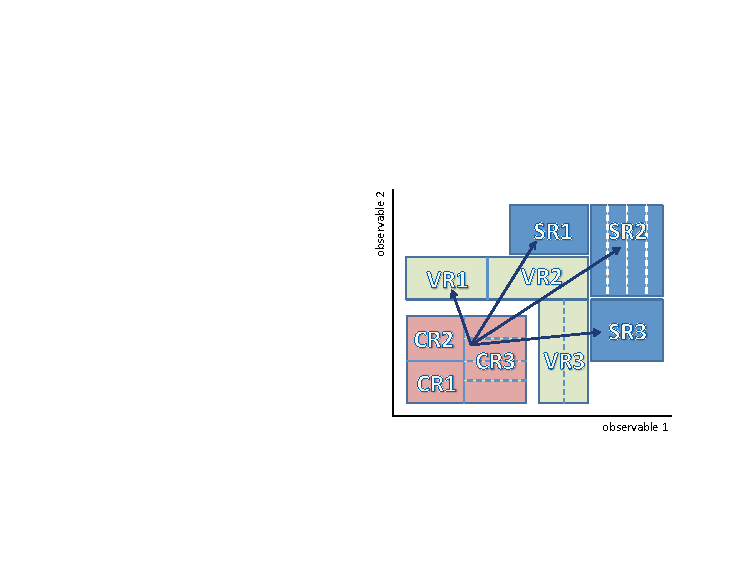
\includegraphics[width=0.55\textwidth]{figures/susy_common/CR_VR}
\caption{Schematic view of the relation between \glspl{cr}, \glspl{vr} and \glspl{vr}. Figure from Ref. \cite{Baak:2014wma}.}
\label{fig:susy_common:CRschema}
\end{figure}
 
In each of the analyses described in the next two chapters, two different analysis strategies are carried out in parallel:
\begin{description}
\item[Cut-and-count] Several \glspl{sr} are designed, each optimized to maximize the discovery significance to a specific region of the phase space, represented by one benchmark model. Cut-and-count \glspl{sr} are useful also to provide simple and powerful model-independent \glspl{ul}, that are easy to re-interpret for signal models different than the ones considered in the analysis. 

\item[Multi-bin] In this case, the \glspl{sr} are non-overlapping. This requirement conflicts with the simple choice of the best selection to maximize the significance, which means that the individual discovery power of each \gls{sr} is smaller than in the case of cut-and-count \glspl{sr}. On the other hand, having non-overlapping \glspl{sr} allows to statistically combine them in the Likelihood fit, leading to a stronger model-dependent expected \gls{ul}. The increase in expected exclusion obtained with the combination of several regions is shown in Section \ref{sec:example_combi}.
 
\end{description}



\section{Background Processes and their modelling}
\label{sec:common_backgrounds}

This section describes the main background processes from the \gls{sm} in the analysis regions and the way they are 
modeled in the analyses discussed in the next two chapters, which are characterized by the selection of events with a high number of b-jets 
and high \met. 
In general, the modelling is based on \gls{mc} simulations for
all the backgrounds, except multi-jet which is emulated with a data-driven technique.
For the main background, pair production of top quark pairs (\ttbar), the shape of the different distributions is obtained from \gls{mc}
but the normalization is data-driven, derived in specifically designed \glspl{cr} and tested in \glspl{vr} as described above.


\subsection{Top quark pair production}

Given the presence of several b-jets in the final state, \ttbar production in association with jets constitutes the main source of \gls{sm} background in all the analysis regions. \ttbar production, which at the \gls{lhc} at 13 TeV has a cross section of $831.8^{+19.8 + 35.1}_{-29.2-35.1}$ pb \cite{Czakon:2013goa}, is mediated by the strong interaction, and it can occur through quark-antiquark annihilation (Fig. \ref{fig:ttbar_prod_qq}) or through gluon-gluon fusion (Fig. \ref{fig:ttbar_prod_gg_1} to \ref{fig:ttbar_prod_gg_3}). When the \gls{lhc} is running at 13 TeV, the threshold fraction of the proton energy that must be carried by each parton in order to have sufficient energy to produce a system of two top quarks 
is about 2.6\%, assuming a top quark mass of 173.1 GeV \cite{Patrignani:2016xqp}. 
At these low fractions, the \gls{partdf} of the gluon is higher than the \gls{partdf} of quarks and much higher than the \gls{partdf} of the antiquarks, so gluon-gluon fusion is the dominant \ttbar production mode at the \gls{lhc}.

\begin{figure}[h]
\centering 
\subfigure[]{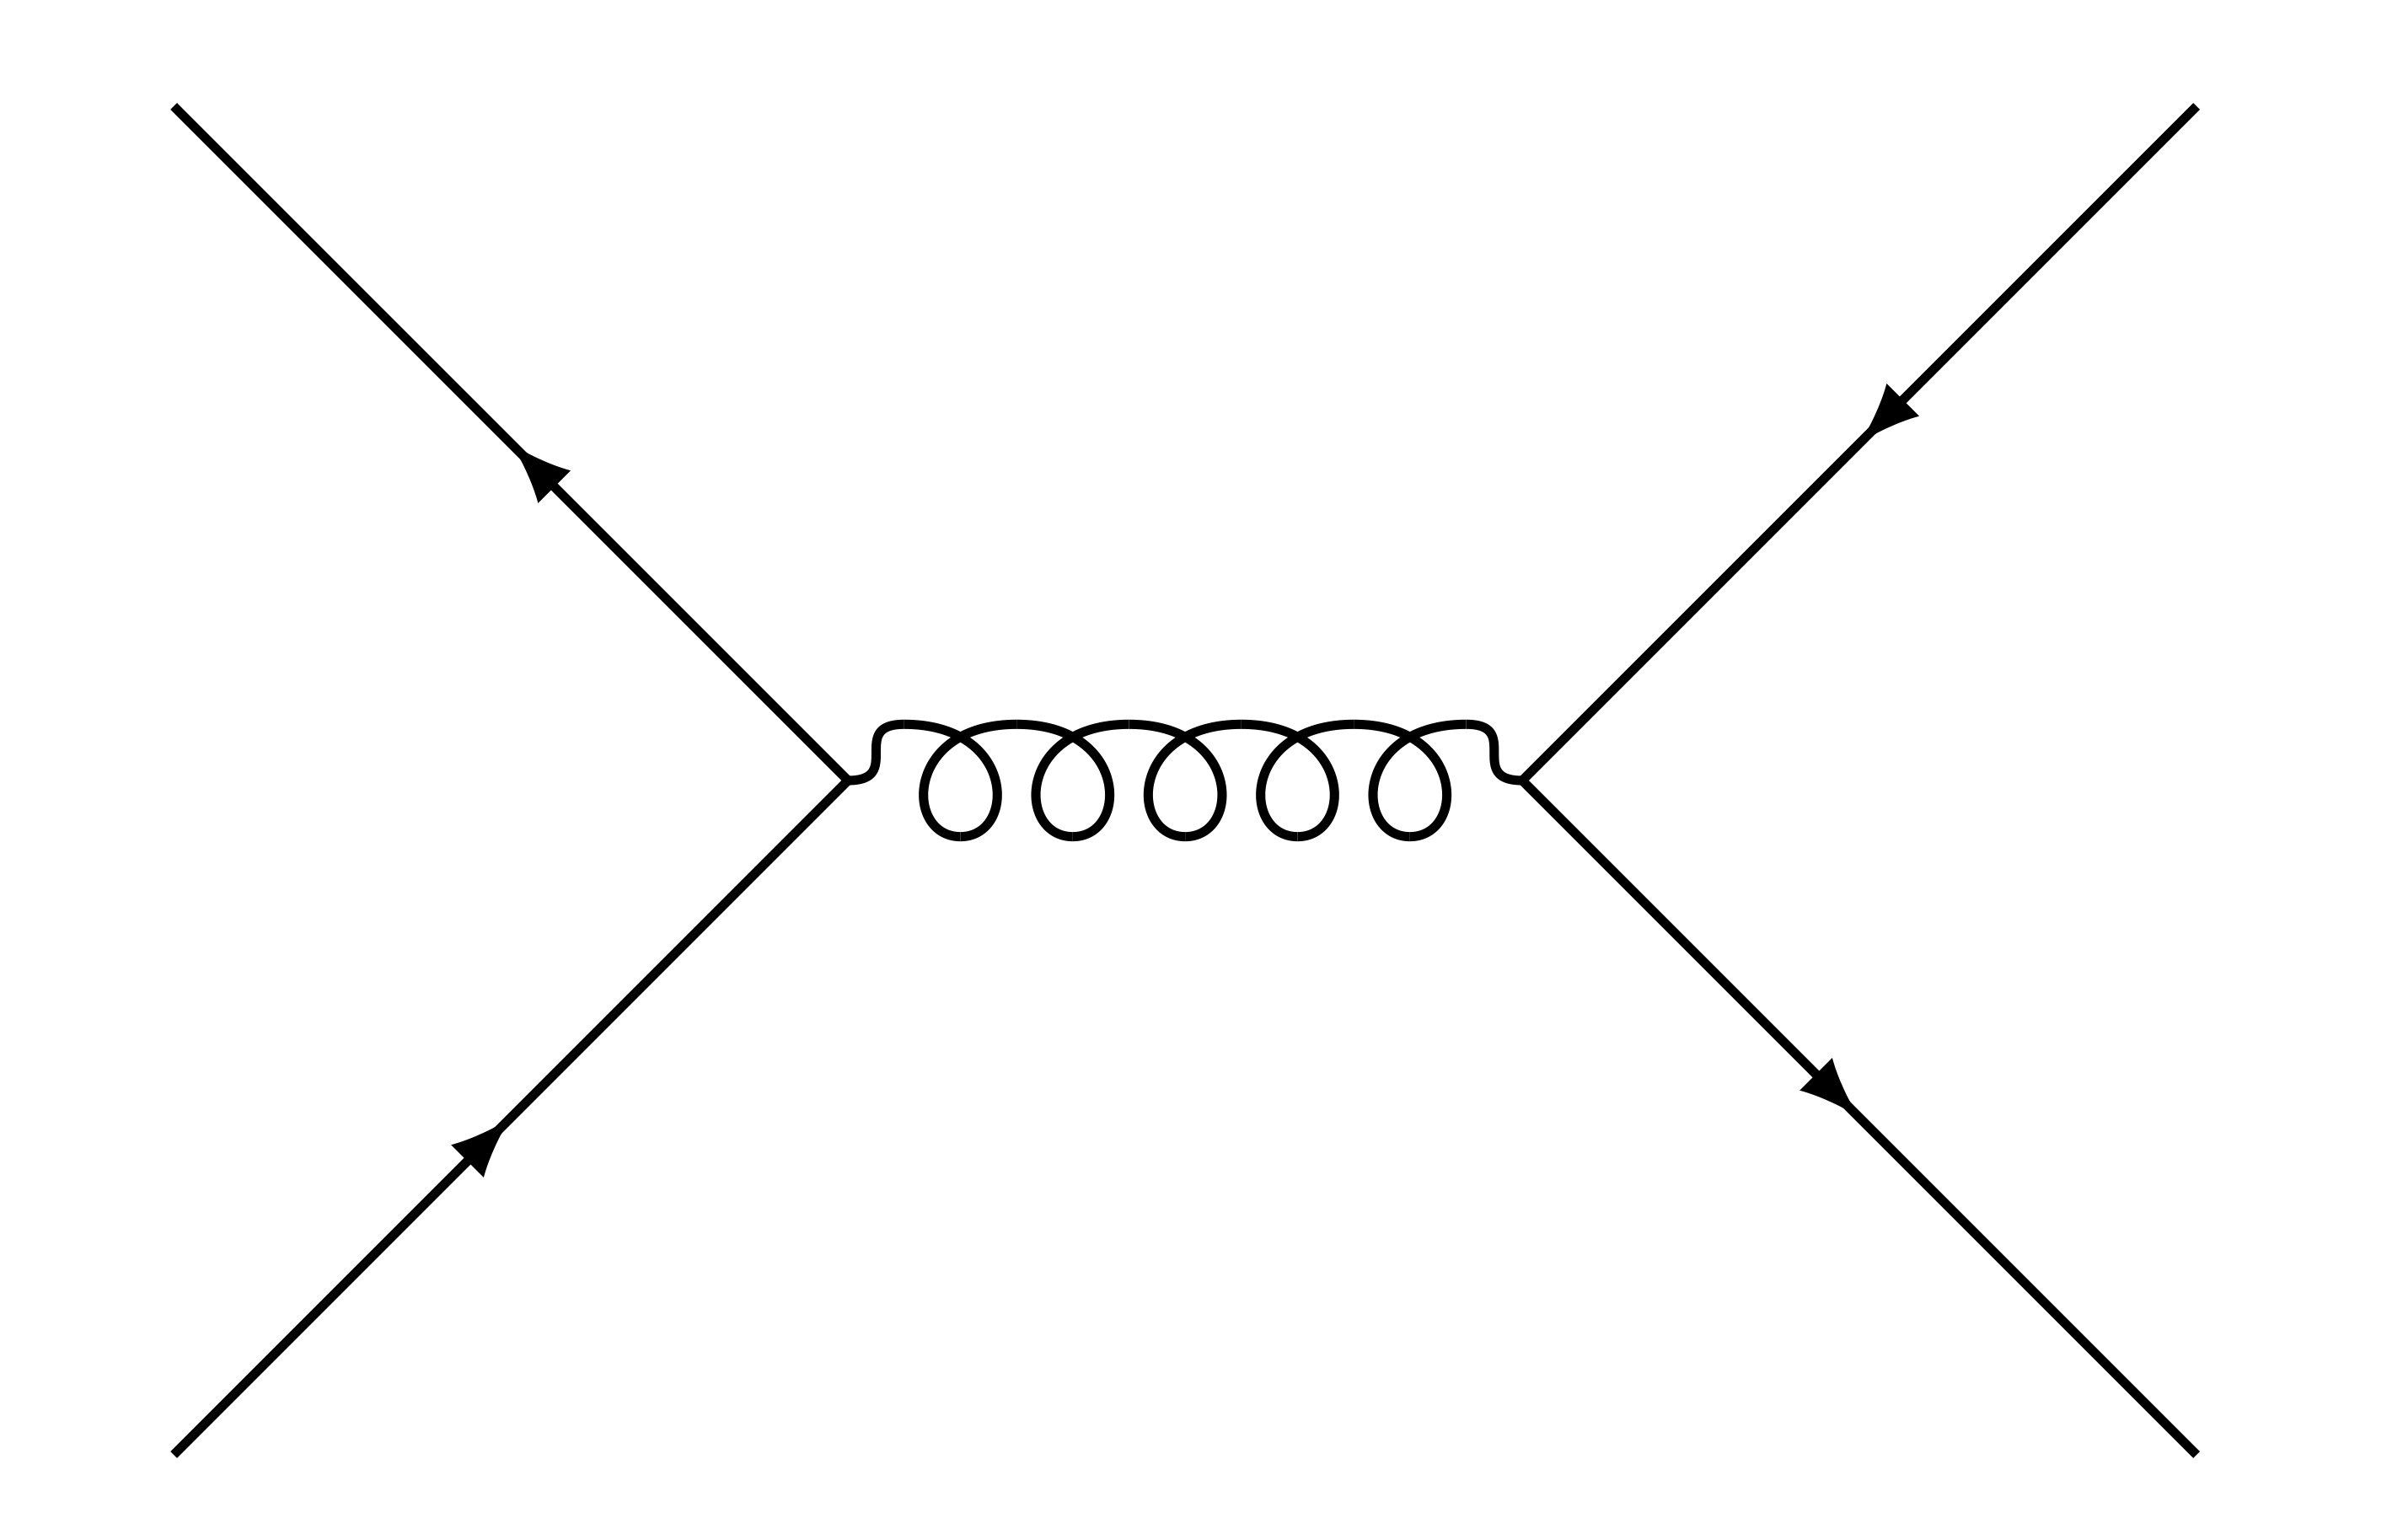
\includegraphics[width=0.3\textwidth]{figures/susy_common/feynman/ttbar_4}\label{fig:ttbar_prod_qq}}\\
\subfigure[]{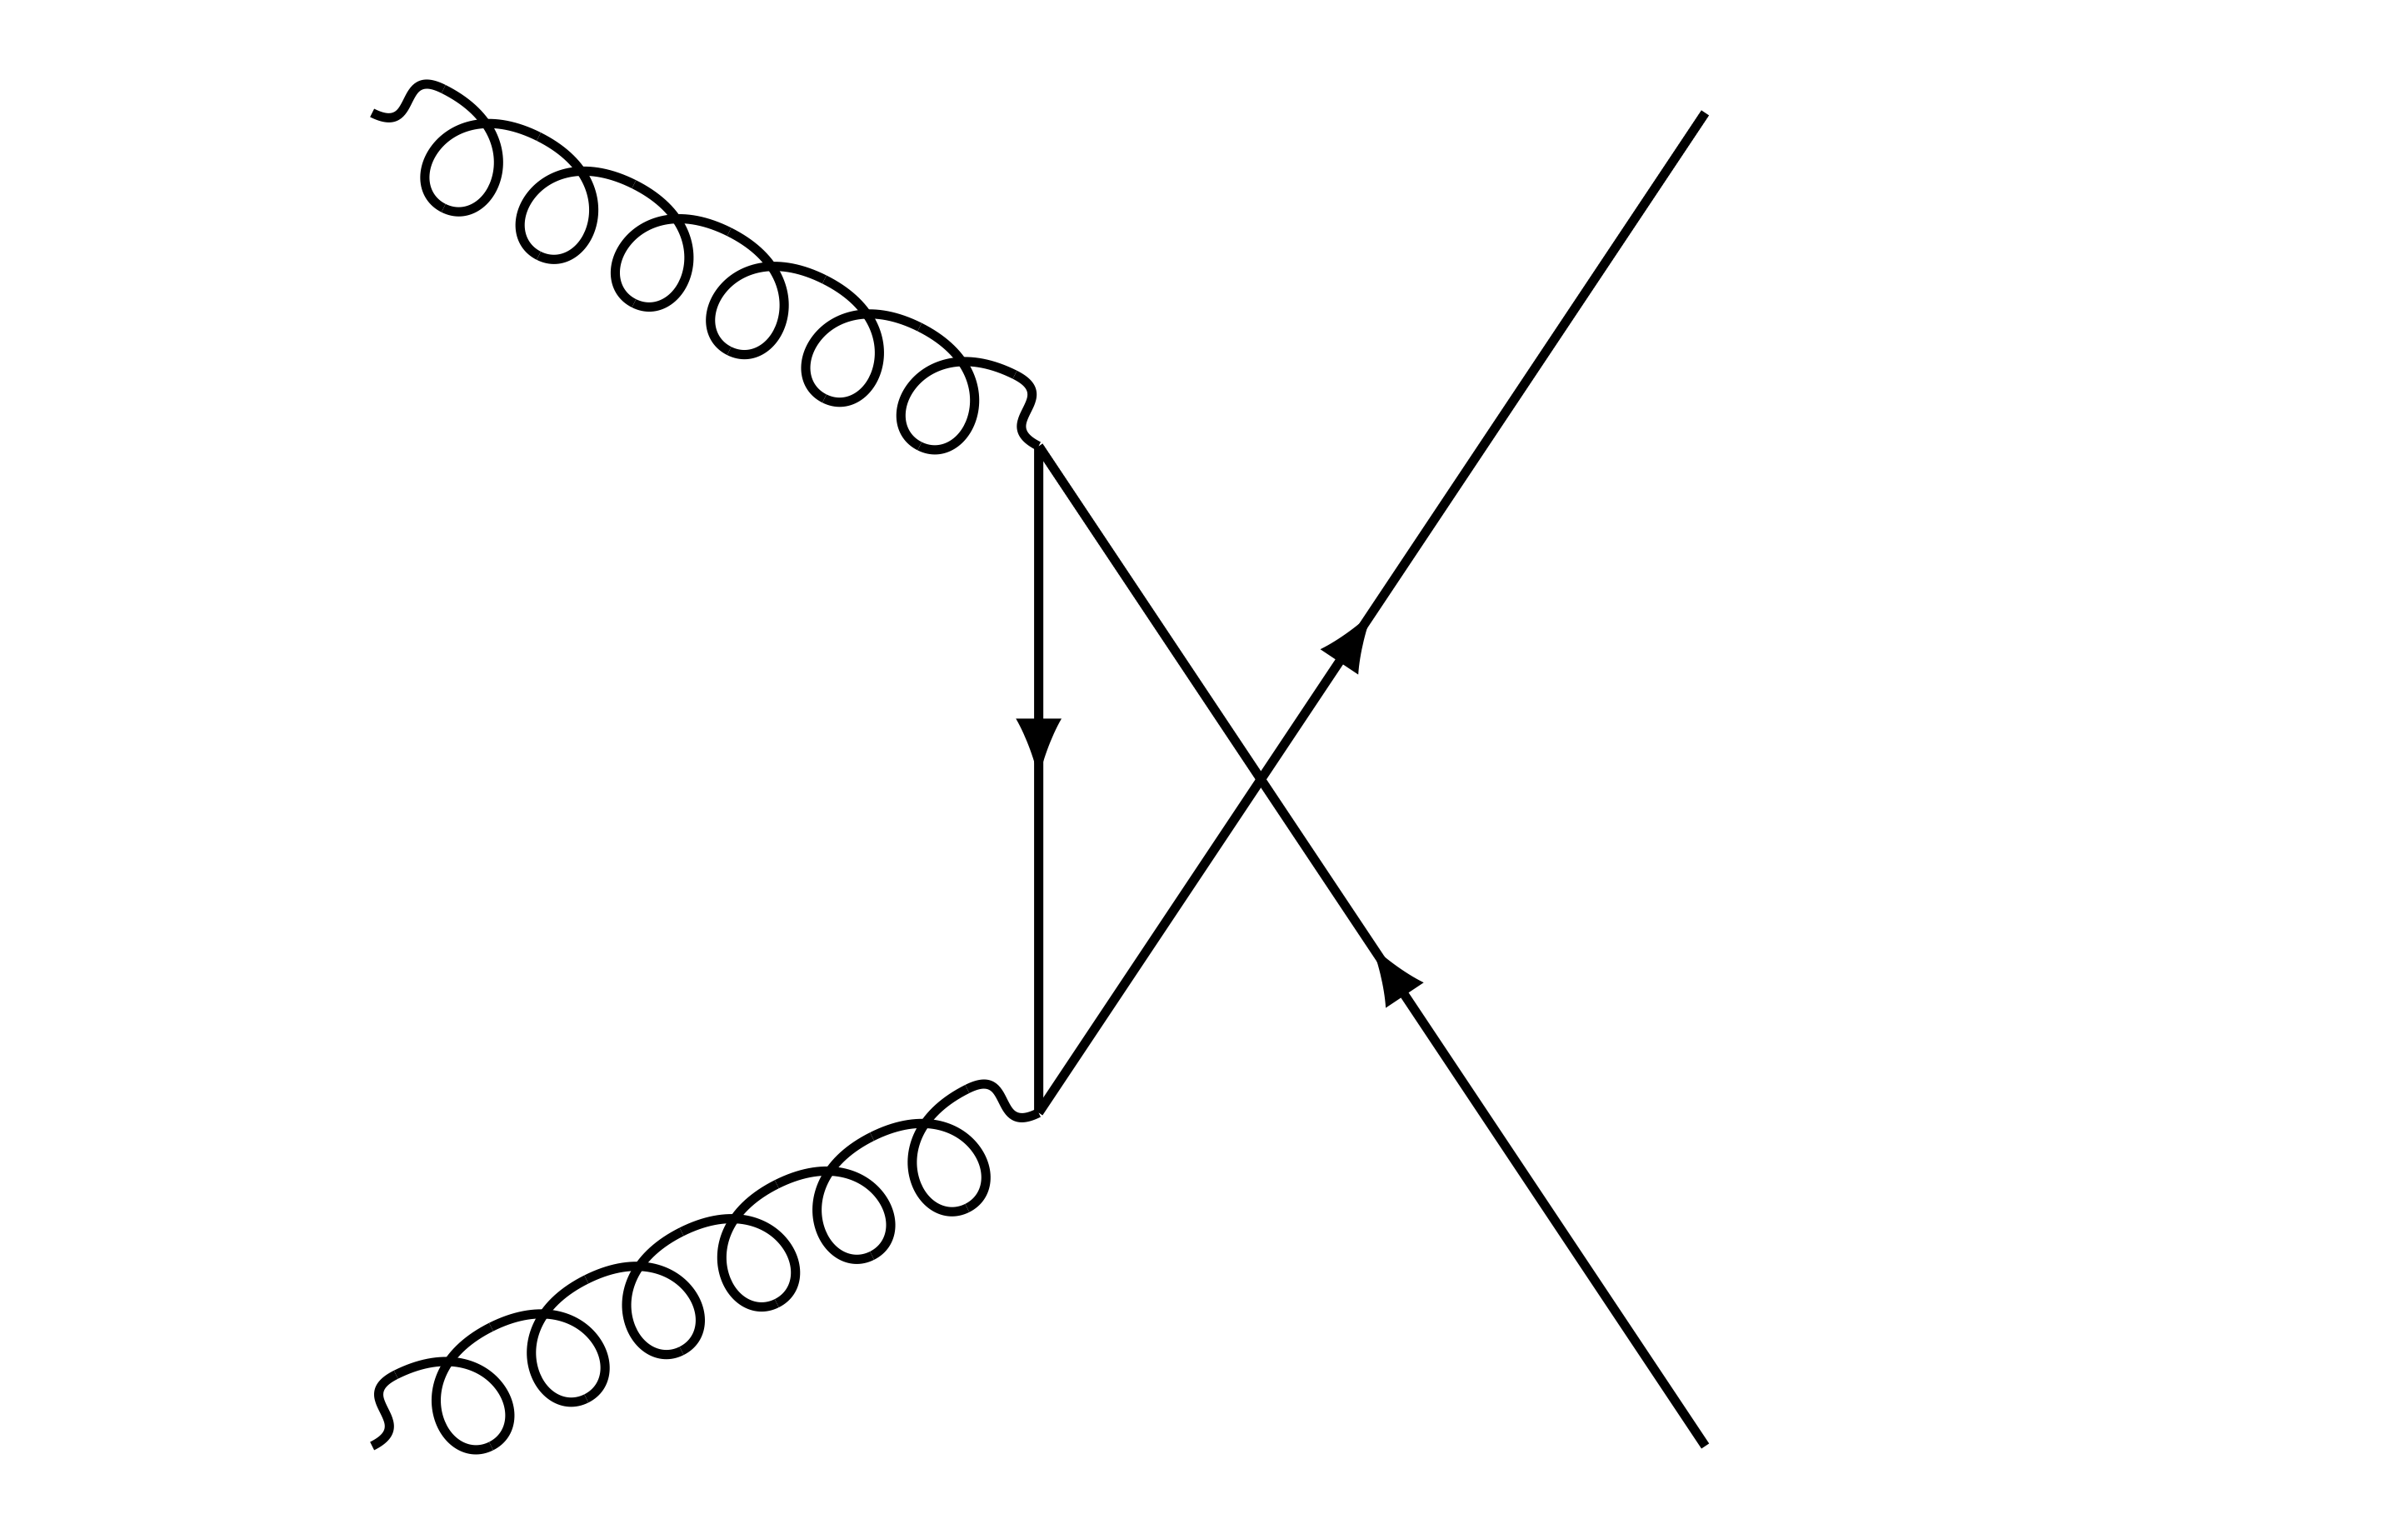
\includegraphics[width=0.3\textwidth]{figures/susy_common/feynman/ttbar_1}\label{fig:ttbar_prod_gg_1}}
\subfigure[]{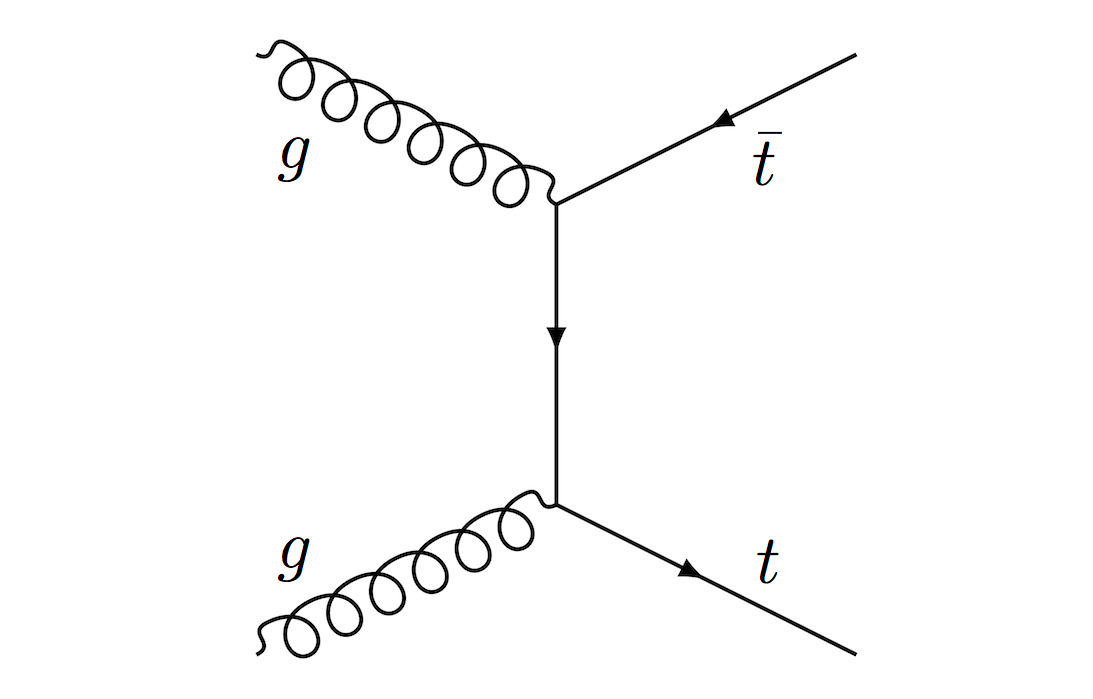
\includegraphics[width=0.3\textwidth]{figures/susy_common/feynman/ttbar_3}\label{fig:ttbar_prod_gg_2}}
\subfigure[]{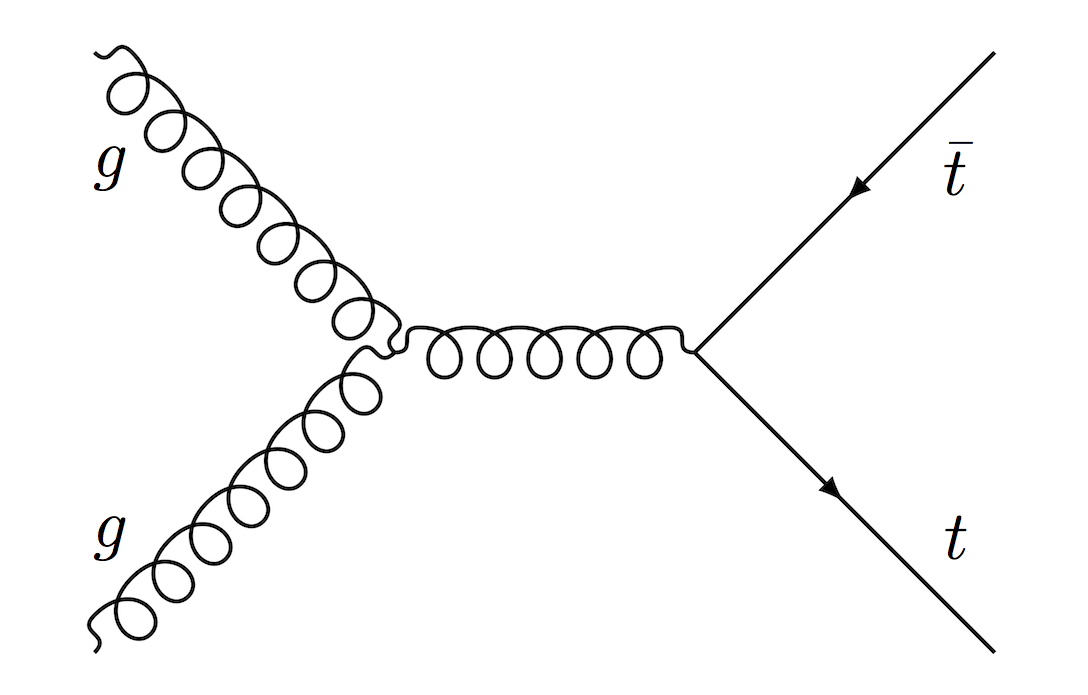
\includegraphics[width=0.3\textwidth]{figures/susy_common/feynman/ttbar_2}\label{fig:ttbar_prod_gg_3}}
\caption{\Gls{lo} Feynman diagram for the production of top quark pairs initiated by \subref{fig:ttbar_prod_qq} quark-antiquark annihilation and \subref{fig:ttbar_prod_gg_1}-\subref{fig:ttbar_prod_gg_3} gluon-gluon fusion.}\label{fig:ttbar_prod}
\end{figure}

In the \gls{sm}, the top quark decays $\approx 99.8$\% of the times to a W boson and a b-quark. 
Beside the pair of b-quarks, that are always present, the final state can be characterized based on the decay of the two W bosons, leading to three different categories:
\begin{description}
\item[Dilepton]  Both W bosons decay to a lepton ($e$, $\mu$, $\tau$) and a neutrino (10.5\%).
\item[Single-lepton] One W boson decays to lepton and neutrino, the other decays hadronically (43.8\%).
\item[All-hadronic] Both W bosons decay hadrinically (45.7\%).
\end{description}

All the analysis regions considered in this thesis have a tight \met selection (the loosest one is $\met > 200$ GeV). Since the all-hadronic component 
of the \ttbar background does not have any neutrino in the final state, it does not fulfill the \met requirement unless one or more jets are not measured correctly; this case produces a negligible background in the analysis regions, and is anyway included in the multi-jet estimate with the jet-smearing method described in Section \ref{sec:jet_smearing}.
The \ttbar components that is dominating the background estimate are the dilepton and single-lepton one, both in the analysis regions that require reconstructed leptons as well as in the analysis regions that have a lepton veto.
In the second case, the dominating component is the single-lepton one, where one lepton is an hadronically decaying tau, has a \pt too low to be reconstructed or falls out of acceptance. 
The \gls{mc} generator used to simulate \ttbar events produced in association with high-\pt jets is \PowhegBox v2 with the CT10 \gls{partdf} set \cite{Lai:2010vv} and interfaced with \PY v6.428 \cite{Sjostrand:2006za} for the \gls{psh} and hadronization. 
The normalization is derived in \glspl{cr} designed to be kinematically as close as possible to the corresponding \glspl{sr} (while being non-overlapping with them by inverting some of the selections), and is expressed in terms of \glspl{sf} relative to the cross section computed with the highest
available accuracy (NNLO+NNLL \cite{Czakon:2011xx}).

\subsubsection{Truth-level classification: \ttbar decays}

When considering events at particle level,
the \gls{mc} information can be used to reconstruct the decay chains that lead to the stable particles in the final state. 
Starting from each top quark in the event, it is possible to follow its decay chain and classify the event first of all into dilepton or single-lepton, or also with a finer classification based on the flavour of the lepton. 
Subsequent decays of the $\tau$ lepton are not considered, and hadronically decaying taus are fully considered as leptons in this classification. 

\subsubsection{Truth-level classification: flavour of the associated jets}

A truth-level classification is in place to study the \ttbar+jets background based on the flavour of the associated jets.
This is done starting from the \gls{mc} information at particle level; stable particles are grouped into jets using the anti-k$_t$ algorithm 
described in Section \ref{sec:obj:jetfinding} with R=0.4; only particle jets with $\pt > 15$ GeV and $|\eta|<2.5$ are considered. 
he flavour of the jet is determined by matching them with the B- and C-hadrons that are in a cone of $\Delta R = 0.4$ from the jet. 
If the event contains at least one jet matched to one or more B-hadrons, excluding the ones originating from the decay of the top quarks, the event 
is classified as \ttbb. Otherwise, if at least one jet is matched to C-hadrons, excluding the ones from the decay of the top quarks or the W bosons, the event is classified as \ttcc. \ttbb and \ttbb events are categorized together as \tthf events, where HF stands for heavy flavour, while the remaining ones are classified as \ttlight.


\subsubsection{Modelling Uncertainties}

The modelling uncertainties on the \ttbar background considered in this thesis are:
\begin{description}
\item[Generator] The uncertainty associated with the choice of a specific \gls{mc} generator are accessed by comparing \PowhegBox with \aNLO, both interfaced with \HWpp v2.7.1 with the UEEE5 underlying-event tune.

\item[Parton shower and hadronization] Also the choice of the generator that emulates the \gls{psh} and the hadronization is associated to an uncertainty, that is evaluated by comparing the nominal sample, generated with \PowhegBox and showered with \PY, to another sample generated again with \PowhegBox but showered with \HWpp v2.7.1. 

\item[Radiation] The systematic uncertainty deriving from the modelling of the \gls{isr} and \gls{fsr} is estimated by comparing samples
generated with \PowhegBox interfaced with two versions of \PY v6.428 with two different settings. One uses the PERUGIA2012radHi tune, has $h_{\rm{dump}}$ parameter set to twice the top mass and the renormalization and factorization scales set to twice the nominal value; these settings lead to an overall larger amount of radiation. The second sample uses a version of \PY with the PERUGIA2012radLo tune, has $h_{\rm{dump}}$ set to the top mass and the renormalization and factorization scales set to half of the nominal value, leading to a description of the event with less additional jets. 

\end{description}

The normalization of \ttbar events is derived in the \glspl{cr}, therefore modelling uncertainties affect only the extrapolation from 
the \gls{cr} to the corresponding \glspl{sr} and \glspl{vr}, and not the overall normalization. 
The modelling uncertainties are therefore estimated by comparing the expected values for the \glspl{tf}, defined as the ratio of expected yields in the \gls{sr} or \gls{vr} over the expected yields in the corresponding \gls{cr}. 

The main limitation for the estimate of the uncertainties is the statistical uncertainty of the \gls{mc} samples for the systematic variations, as these samples have in general less simulated events than the nominal sample. 
More statistics is available at particle level, where the simulation of the interaction of the particles with the detector and the following event reconstruction (discussed in Section \ref{sec:detsim}) is not performed, so the evaluation of the \ttbar modelling uncertainties is carried out 
comparing samples at particle level, with the assumption that the detector simulation has a similar effect on all the samples, 
independently of the \gls{mc} generator used. Two further strategies are in place to allow enough statistics in the comparison of the different samples. 
One consists in relaxing or removing some selections to both the \glspl{cr} and the corresponding \glspl{sr}/\glspl{vr}. 
Another is to substitute the selection on the number of b-jets with truth-tagging, described in the next section.

\subsubsection{Truth Tagging}

With truth tagging, instead of keeping only the events that satisfy a certain criterion on the number of b-jets, all the events are kept and weighted. The weight is the probability that, out of all the jets in the event,
a certain number pass the b-tagging identification.
A different weight is computed for each b-tagging requirement, for example the probability for the event to have at least three b-tagged jets will be different form the probability of having exactly two. 
For each jet, the probability to be b-tagged can be expressed as a function of the jet flavour ($f$), \pt and $\eta$:

\begin{equation}
\varepsilon \left(f,|\eta|,p_{\mathrm{T}}\right) \; .
\label{eq:susy_common:btageff}
\end{equation}

\noindent If an event has $N$ jets, the probability of containing exactly one $b$-tag jet can be expressed as:
\begin{equation}
        P_{=1} = \sum\limits_{i=1}^N \left( \varepsilon_{i} \prod\limits_{i \neq j} \left( 1 - \varepsilon_{j} \right) \right) \,
\end{equation}

\noindent and in the same way, we can compute the probability for an inclusive b-tagging selection:
\begin{equation}
 \begin{split}
        P_{=0} &= \prod\limits_{i=1}^N \left( 1 - \varepsilon_{j} \right) \; ,\\
        P_{\geq 1} &= 1 - P_{=0} \; .
 \end{split}
\end{equation} 
 
\noindent This procedure can be extended to an arbitrary number of b-tagged jets by summing over all the possible permutations that lead to the desired number of b-tagged jets ($n$) to derive the exclusive probability and then subtract it from the $P_{\geq n}$ probability to have the inclusive probability for $\geq n+1$ b-tagged jets.
 
Beside decreasing the statistical uncertainty on the expected number of events, the other advantage of using truth tagging on particle-level samples is that it allows to emulate the reconstruction-level efficiency of the b-tagging algorithm: 
at particle-level a jet is considered a b-tagged if it is matched to a b-quark in the \gls{mc} record within a certain cone. This criterion has 
almost 100\% efficiency for real b-jets, and it leads to a null mistag rate. Instead with truth tagging, if the efficiency map used in Equation \ref{eq:susy_common:btageff} corresponds to the b-tagging efficiency measured for reconstructed jets, 
it is possible to obtain the same efficiency to a b-tagging selection as in a reconstructed-level analysis. 

Some analysis variables are build using explicitly the kinematic characteristics of the b-tagged jets, for example the invariant mass of a $b$-$\bar{b}$ system. The truth tagging method allows to choose which jets in the event should be considered as b-tagged: in an event with $N$ jets, each permutation with a $n$ jets considered as b-tagged and $N-n$ jets considered as non b-tagged contributed is characterized by an individual weight $w_i$. If we define $S$ the sum of all these individual weights, a pseudo-random number generated with uniform probability between 0 and $S$ will indicate which permutation to choose and consequently which jets to consider as b-tagged; this procedure is illustrated in Figure \ref{fig:susy_common_trf_perm}. 

\begin{figure}[h]
\centering 
%\subfigure[]{
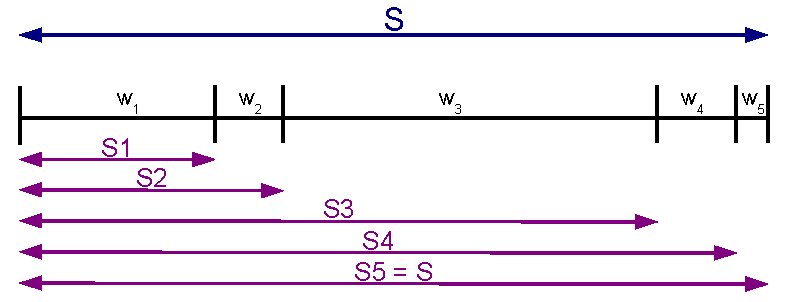
\includegraphics[width=0.6\textwidth]{figures/susy_common/trf_perm}
%}
\caption{Example schema to choose the selected permutation with truth tagging.}\label{fig:susy_common_trf_perm}
\end{figure}


\subsection{Single top quark production}

While the production of a \ttbar pair is mediated by strong interaction, in the case of a single top quark the production occurs through electroweak 
couplings. There are three possible production channels, illustrated in Fig. \ref{fig:single_top_prod}: the Wt-channel, where a top quark and a W boson are produced, the t-channel, and the s-channel. 

\begin{figure}[h]
\centering 
\subfigure[]{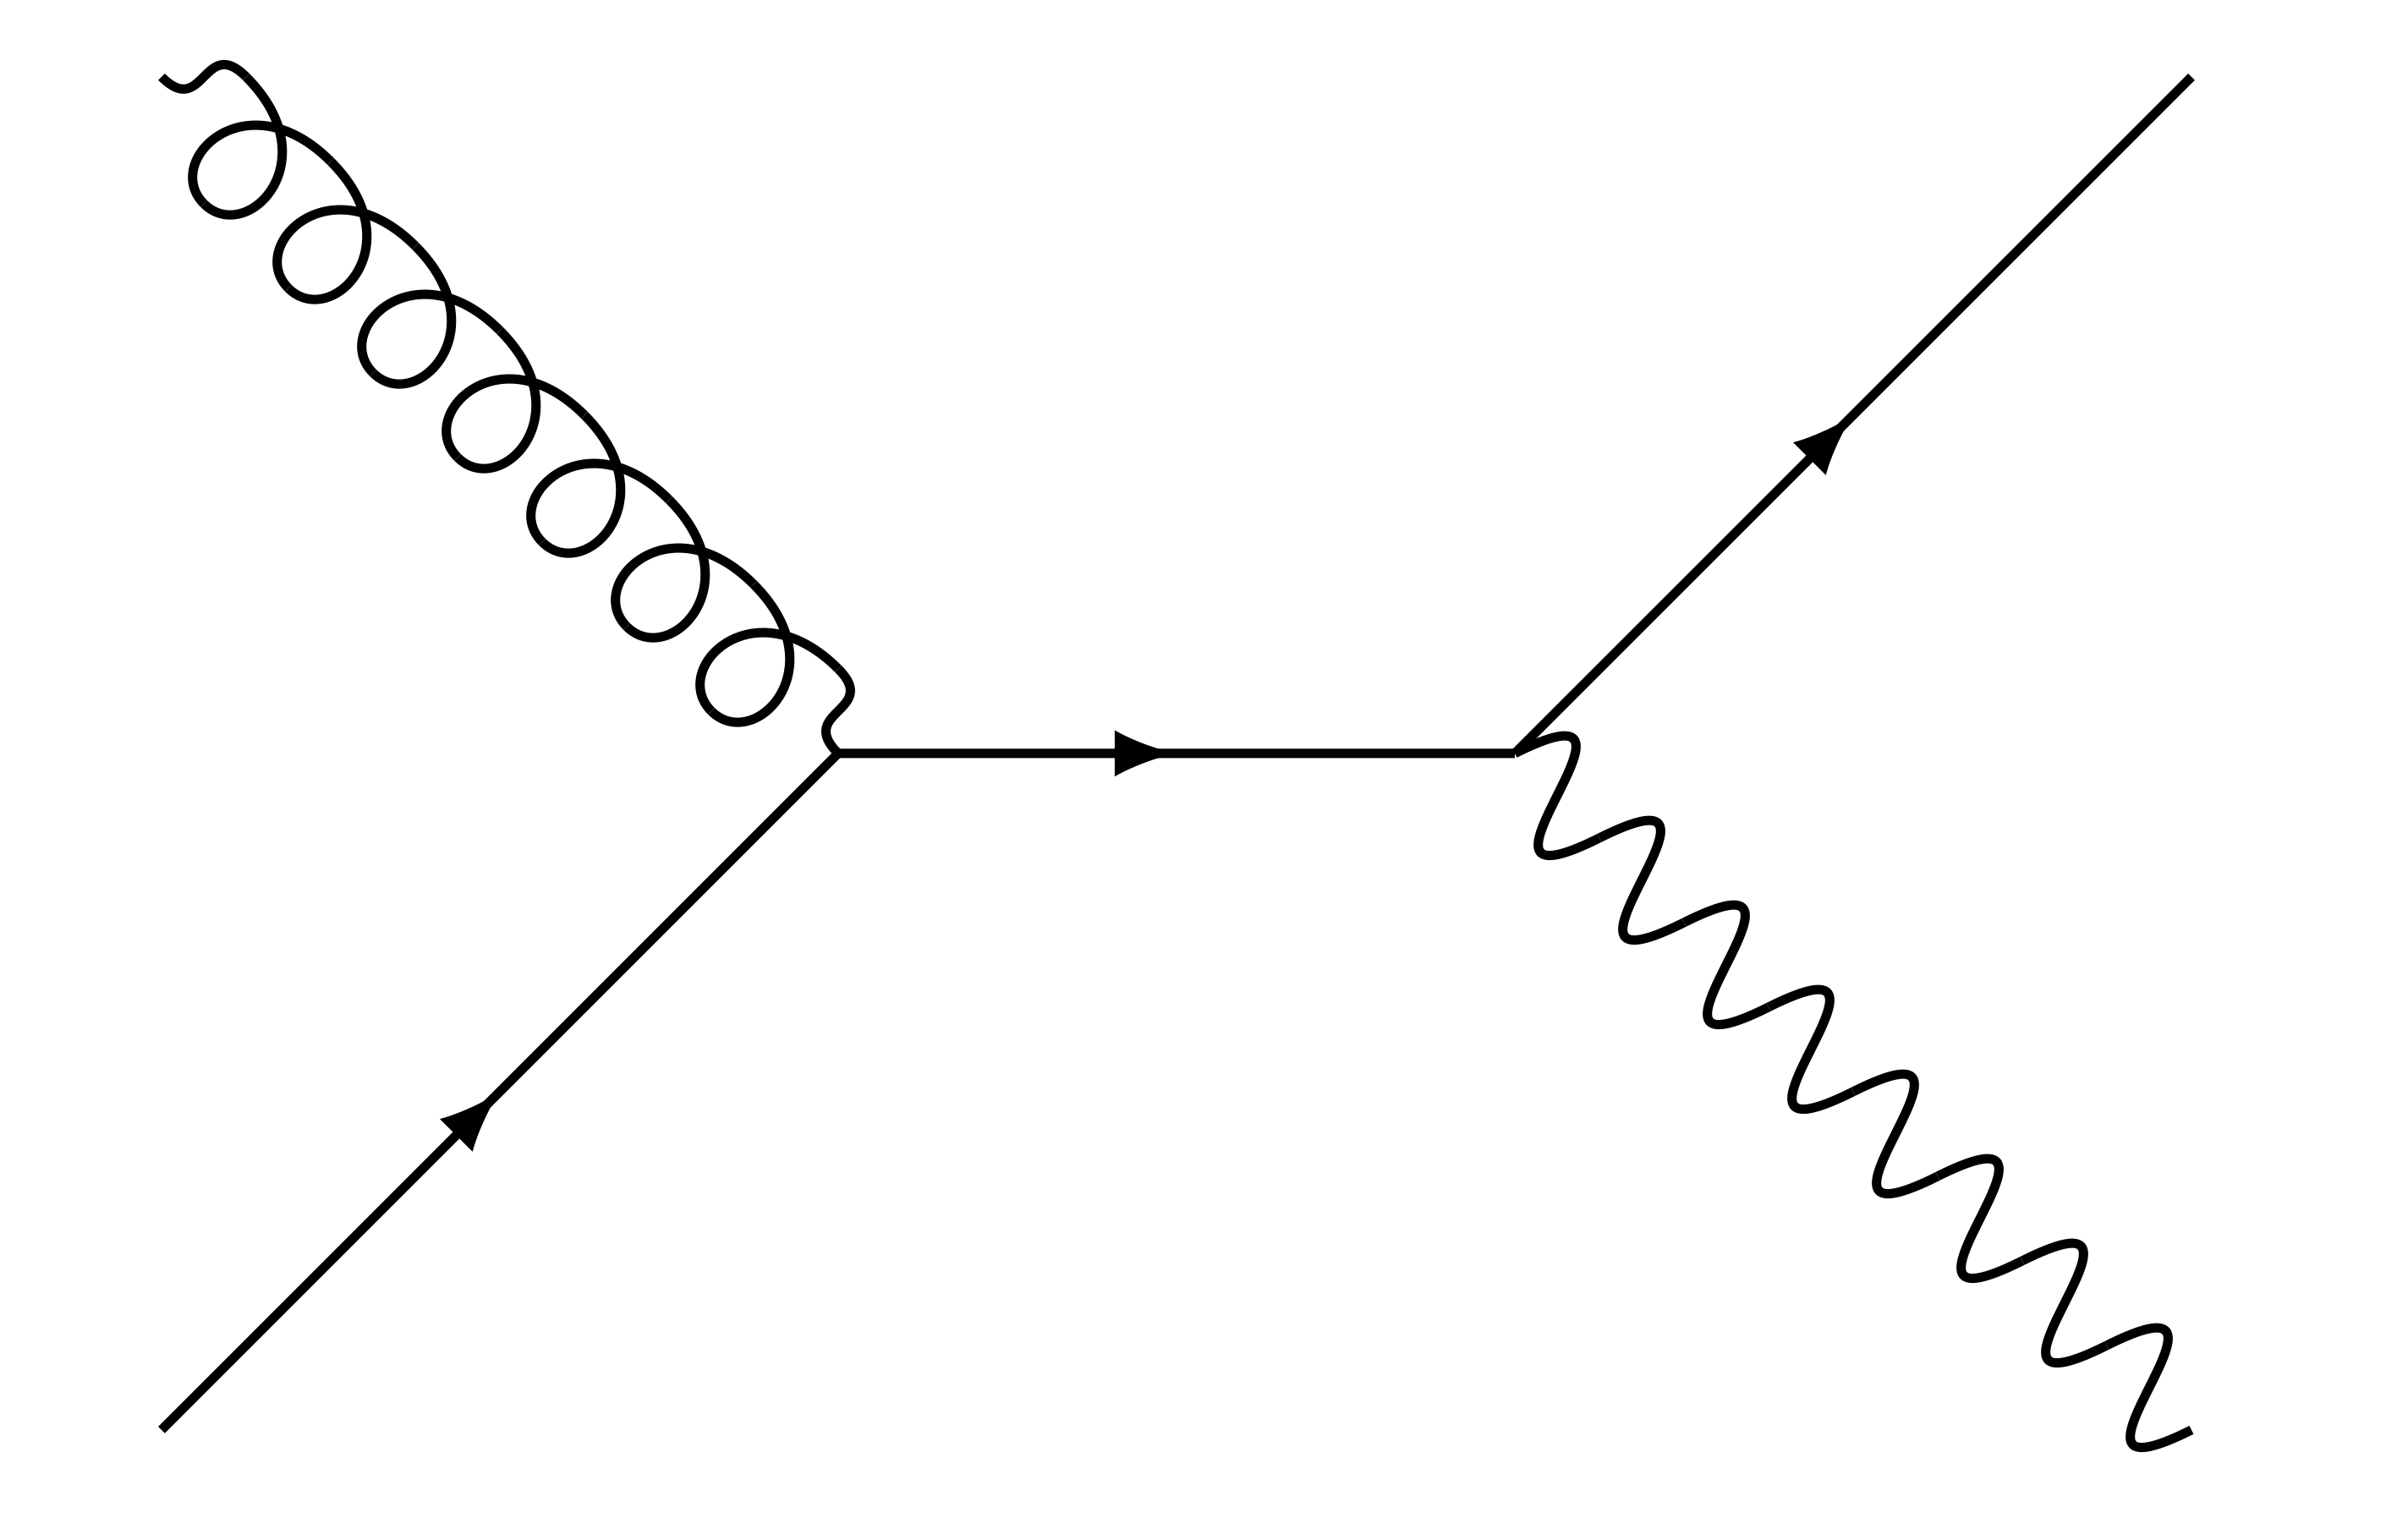
\includegraphics[width=0.3\textwidth]{figures/susy_common/feynman/st_2}\label{fig:st_prod_Wt1}}
\subfigure[]{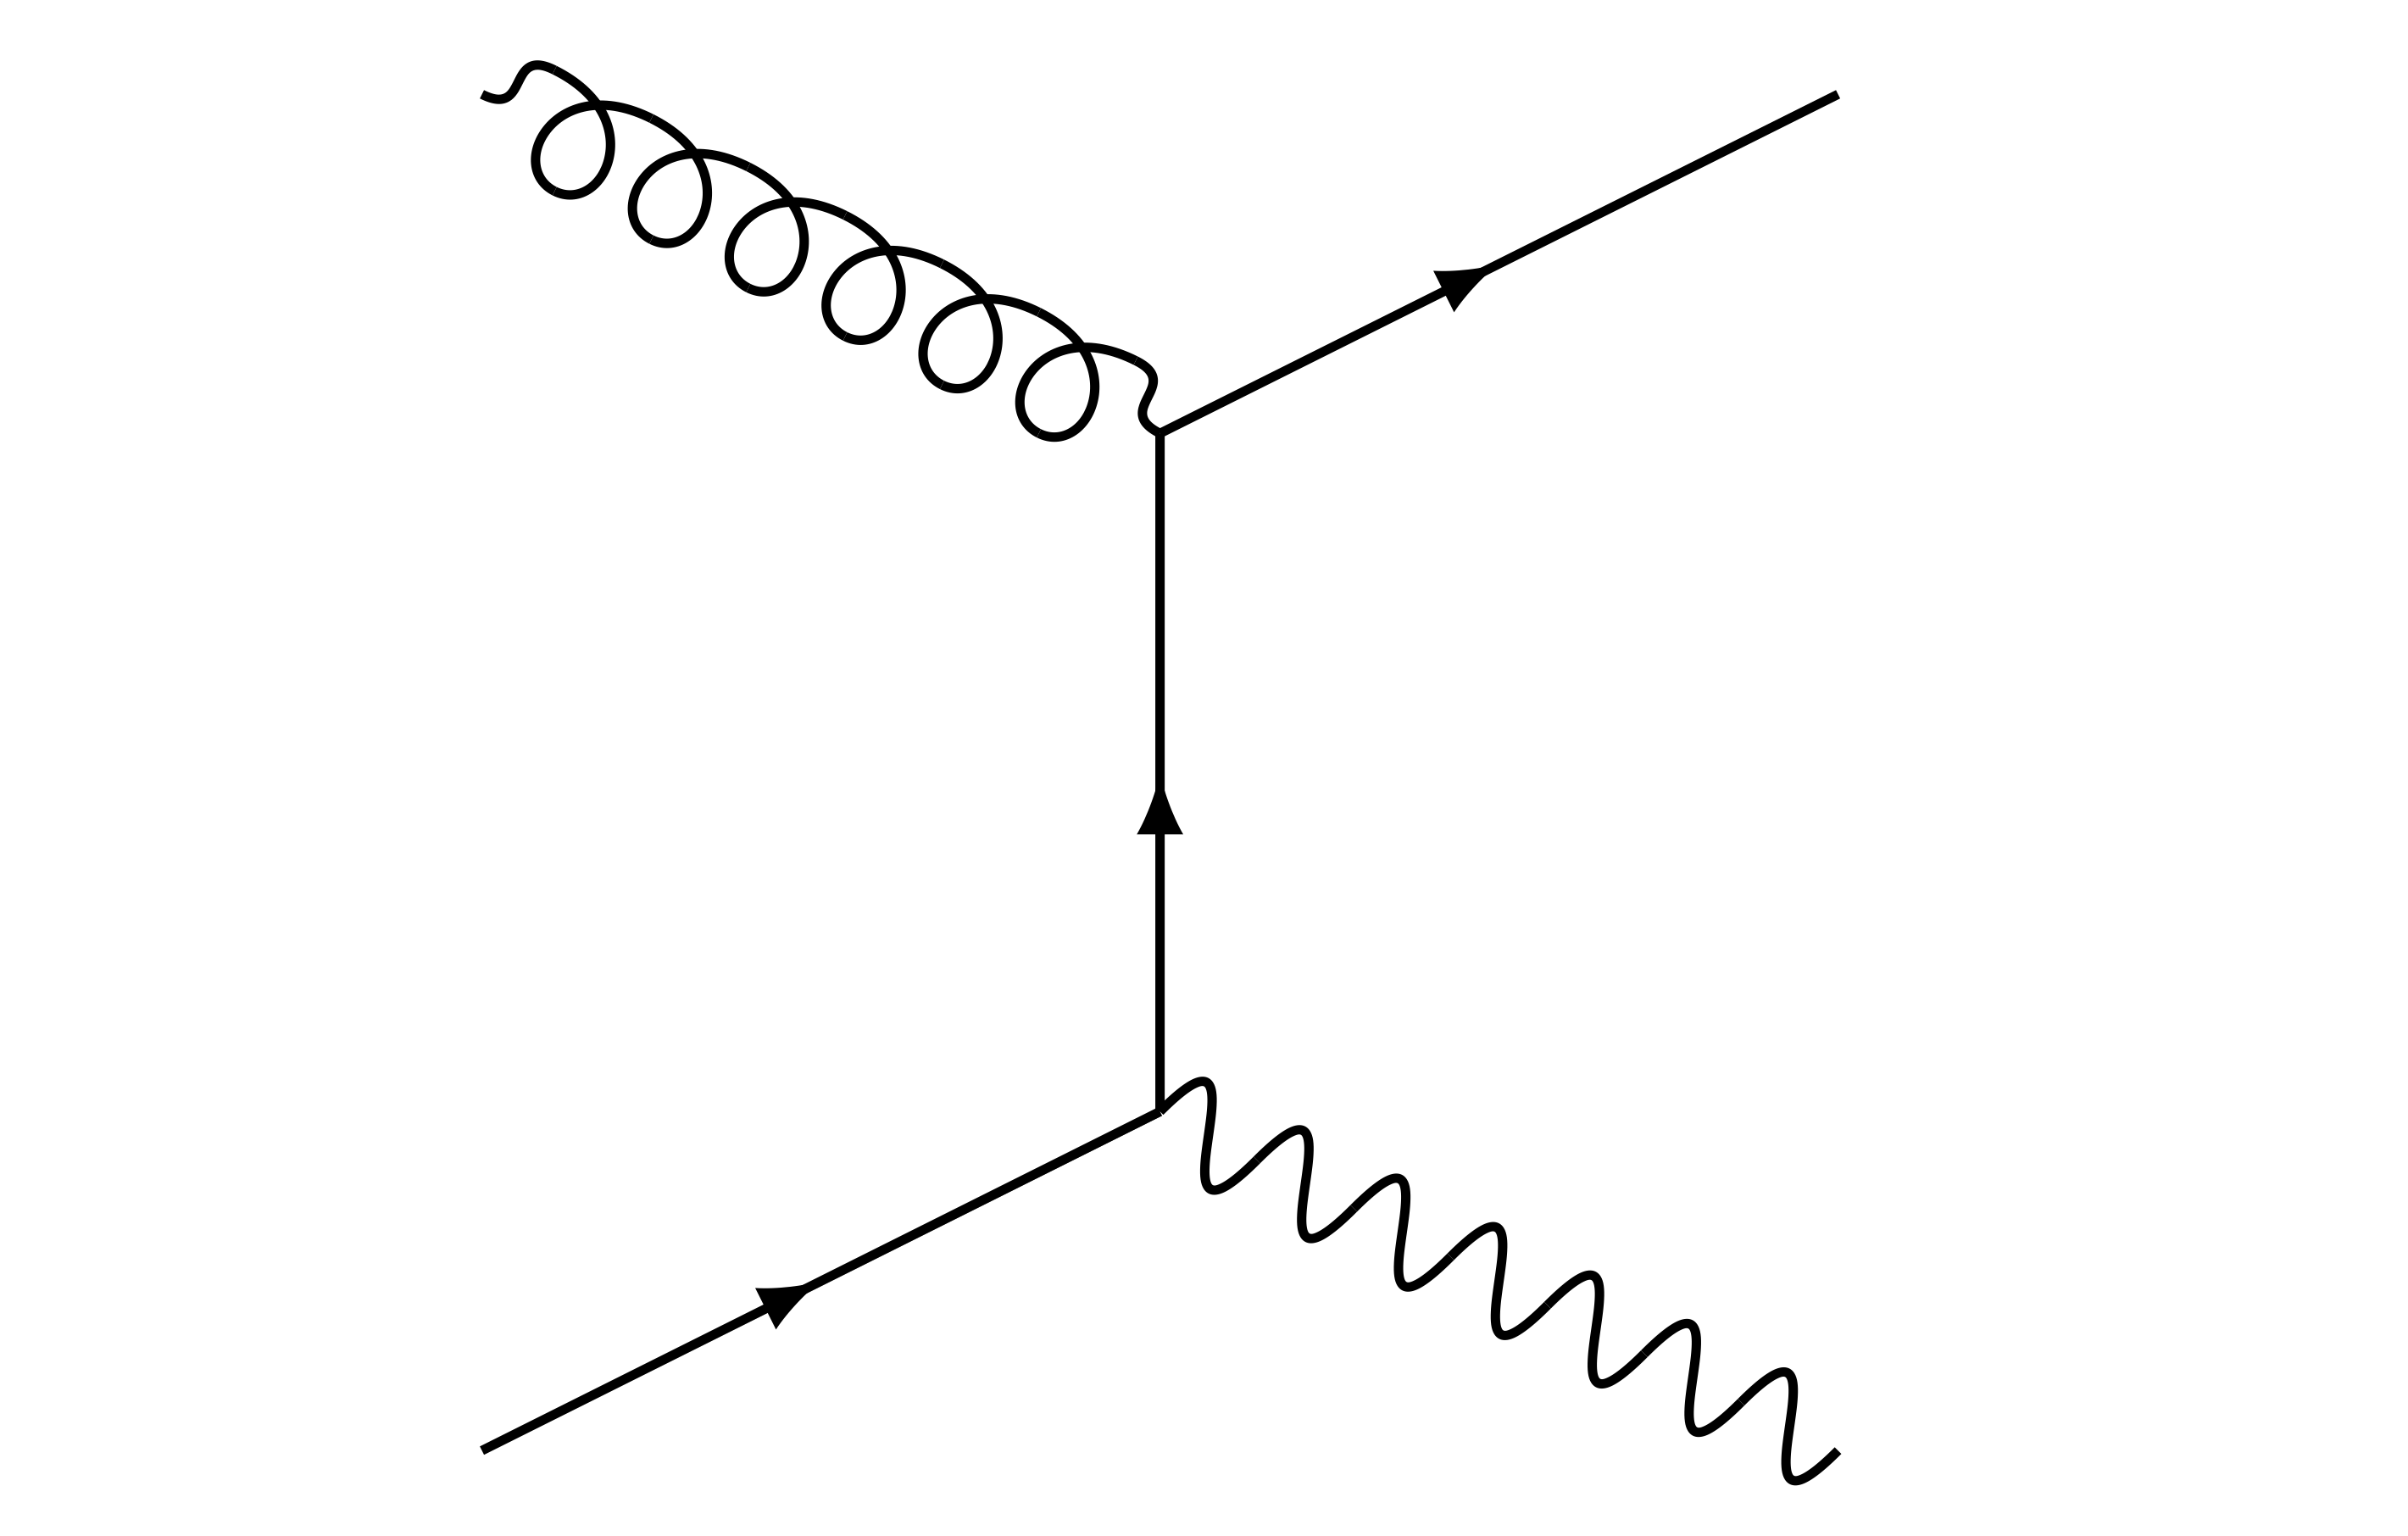
\includegraphics[width=0.3\textwidth]{figures/susy_common/feynman/st_3}\label{fig:st_prod_Wt2}} \\
\subfigure[]{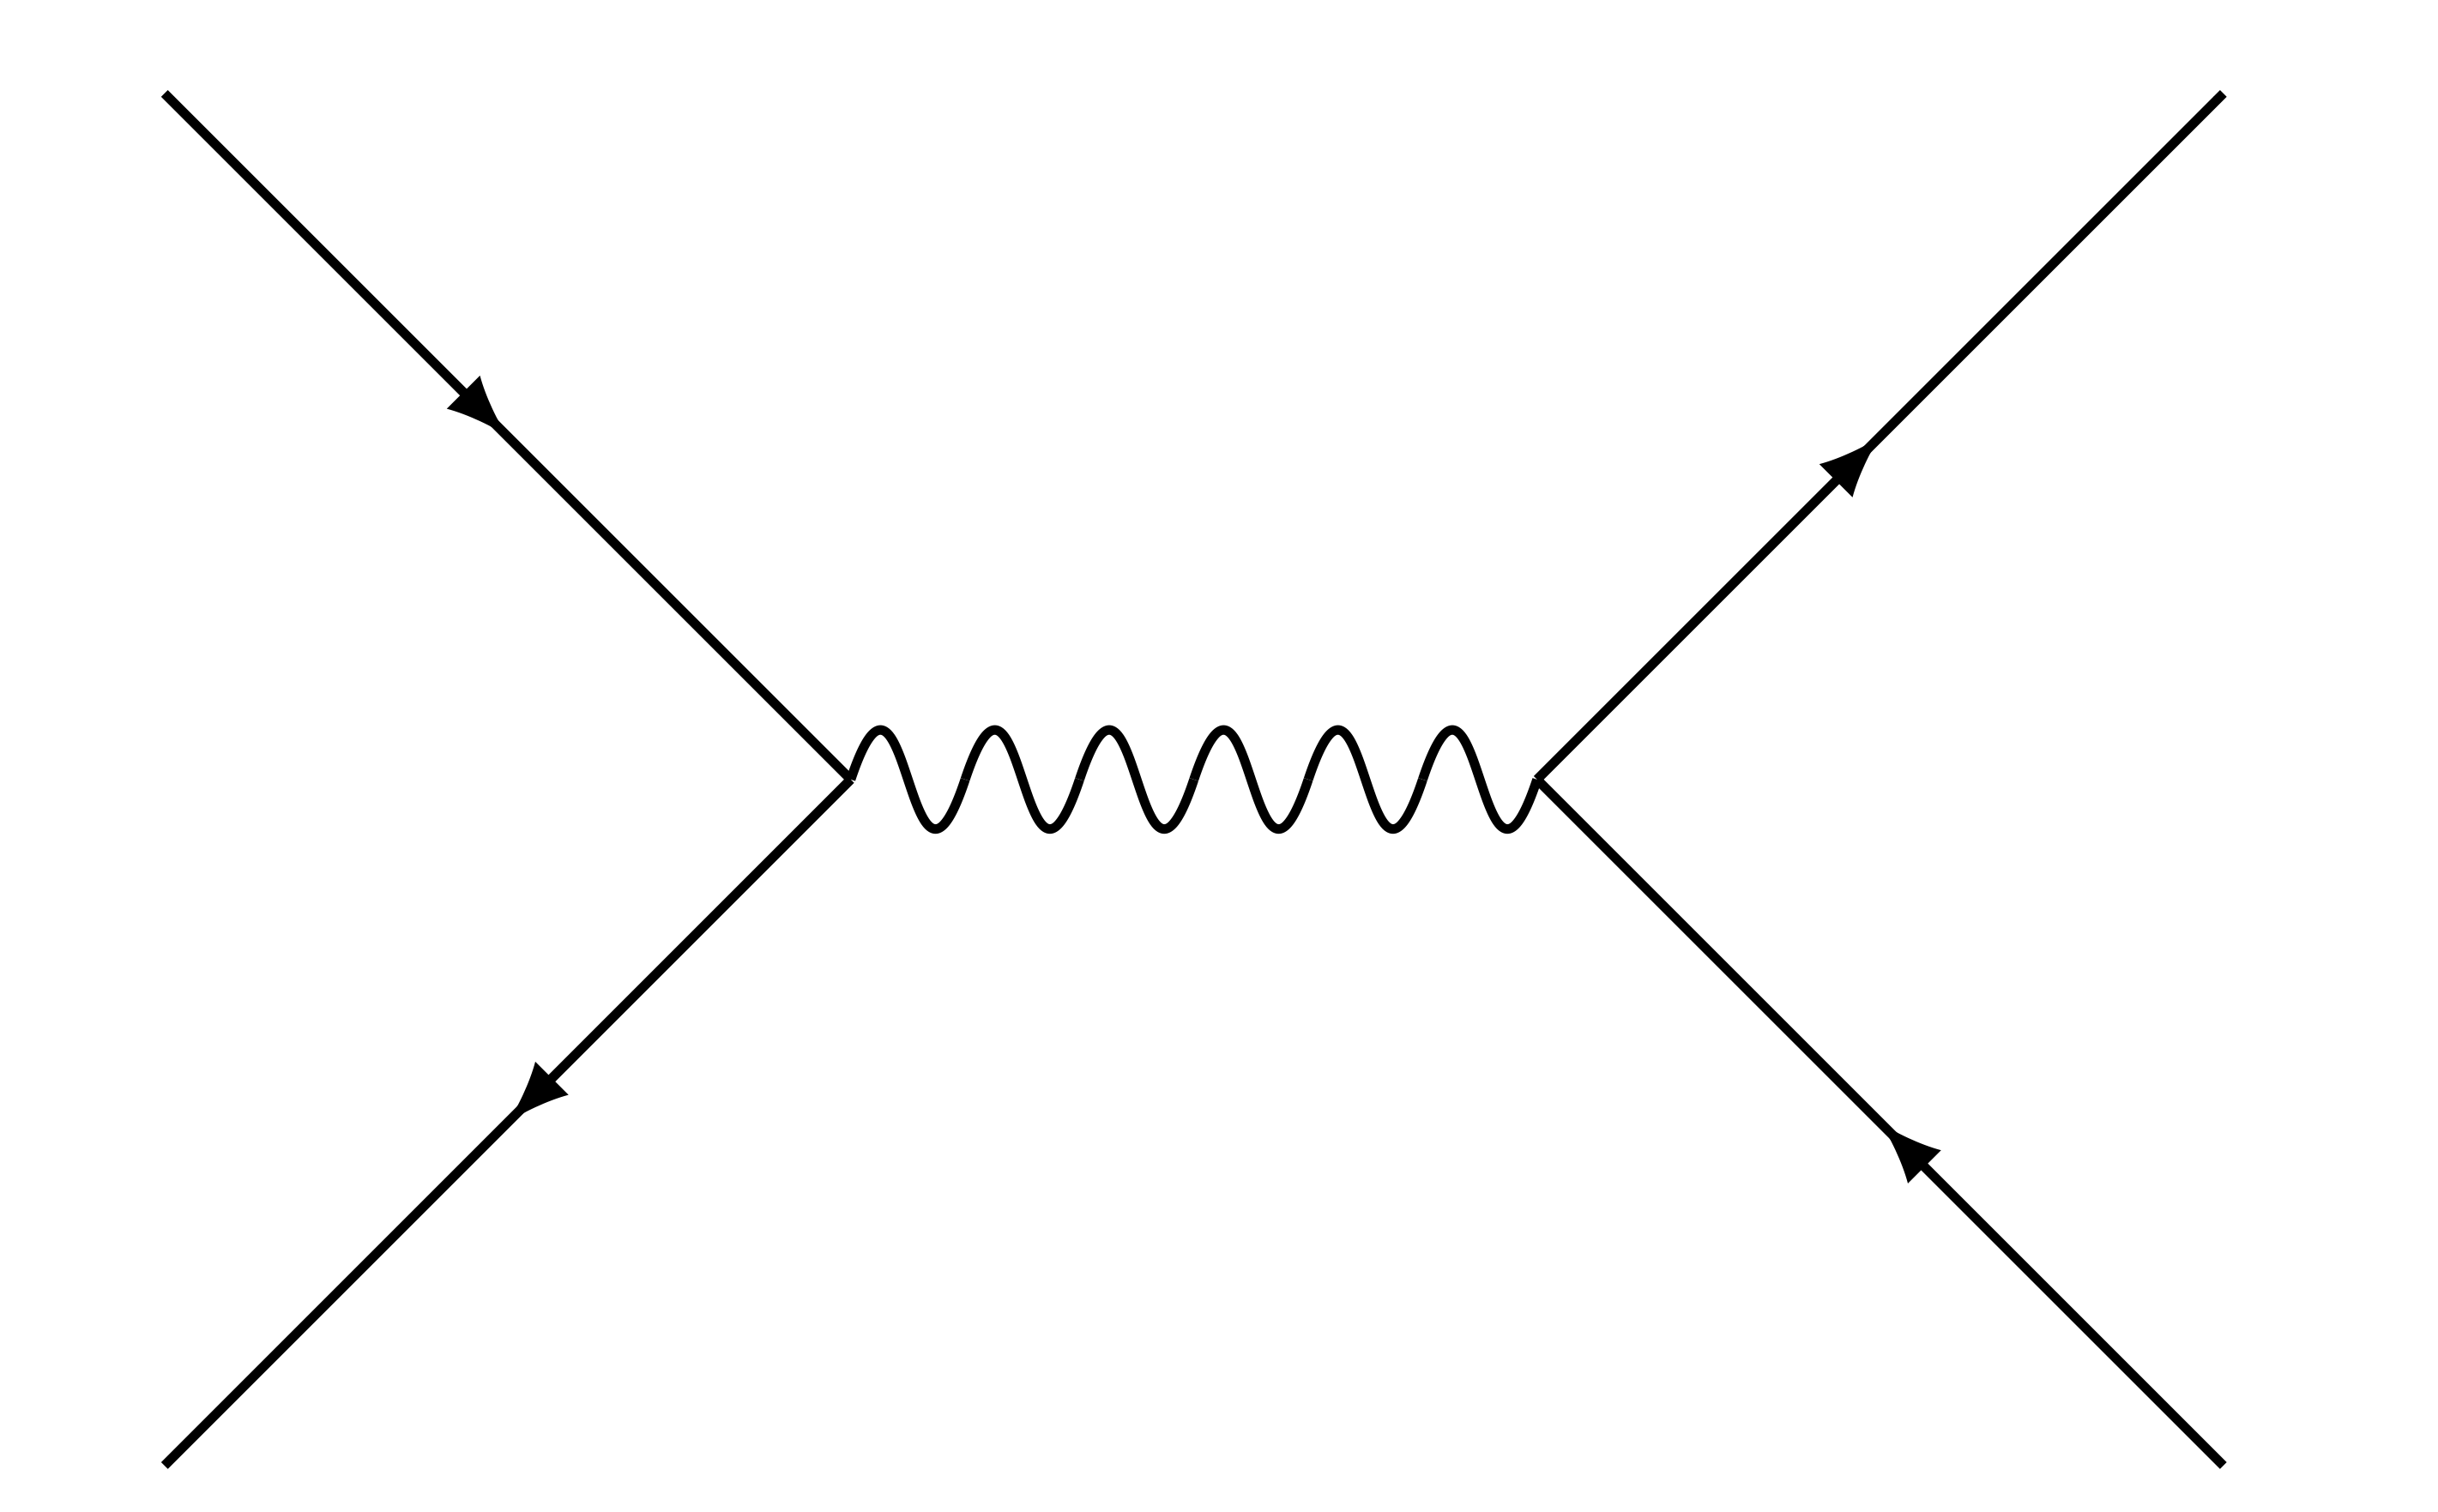
\includegraphics[width=0.3\textwidth]{figures/susy_common/feynman/st_4}\label{fig:st_prod_3}}
\subfigure[]{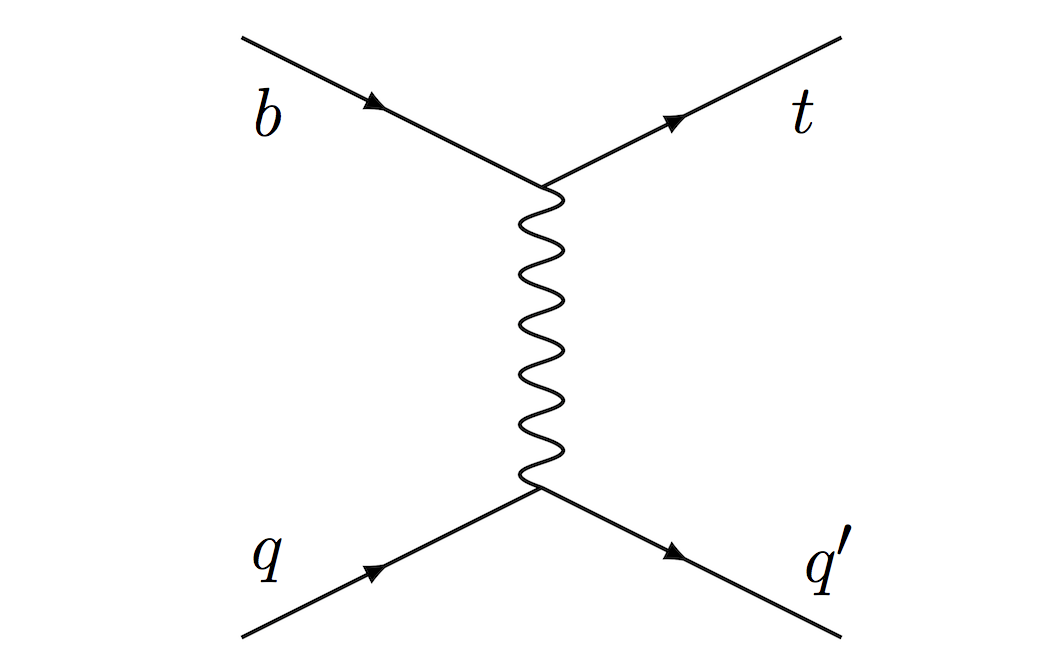
\includegraphics[width=0.3\textwidth]{figures/susy_common/feynman/st_5}\label{fig:st_prod_4}}
\caption{\Gls{lo} Feynman diagram for single top production. \subref{fig:st_prod_Wt1}-\subref{fig:st_prod_Wt2} Wt-channel. 
\subref{fig:st_prod_Wt2} s-channel. \subref{fig:st_prod_4} t-channel.}\label{fig:single_top_prod}
\end{figure}

\subsection{Vector Boson in Association with Jets}


\begin{figure}[h]
\centering 
\subfigure[]{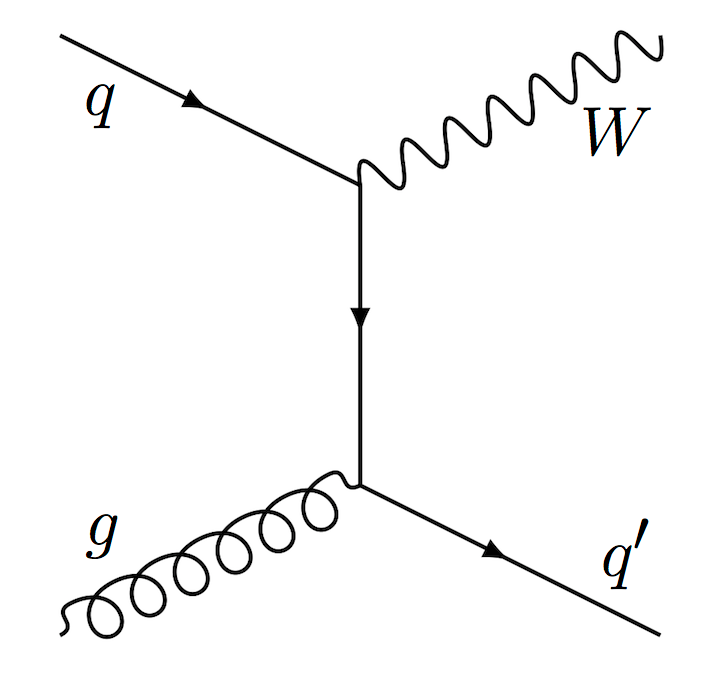
\includegraphics[width=0.25\textwidth]{figures/susy_common/feynman/W_1}\label{fig:W_prod_1}}
\subfigure[]{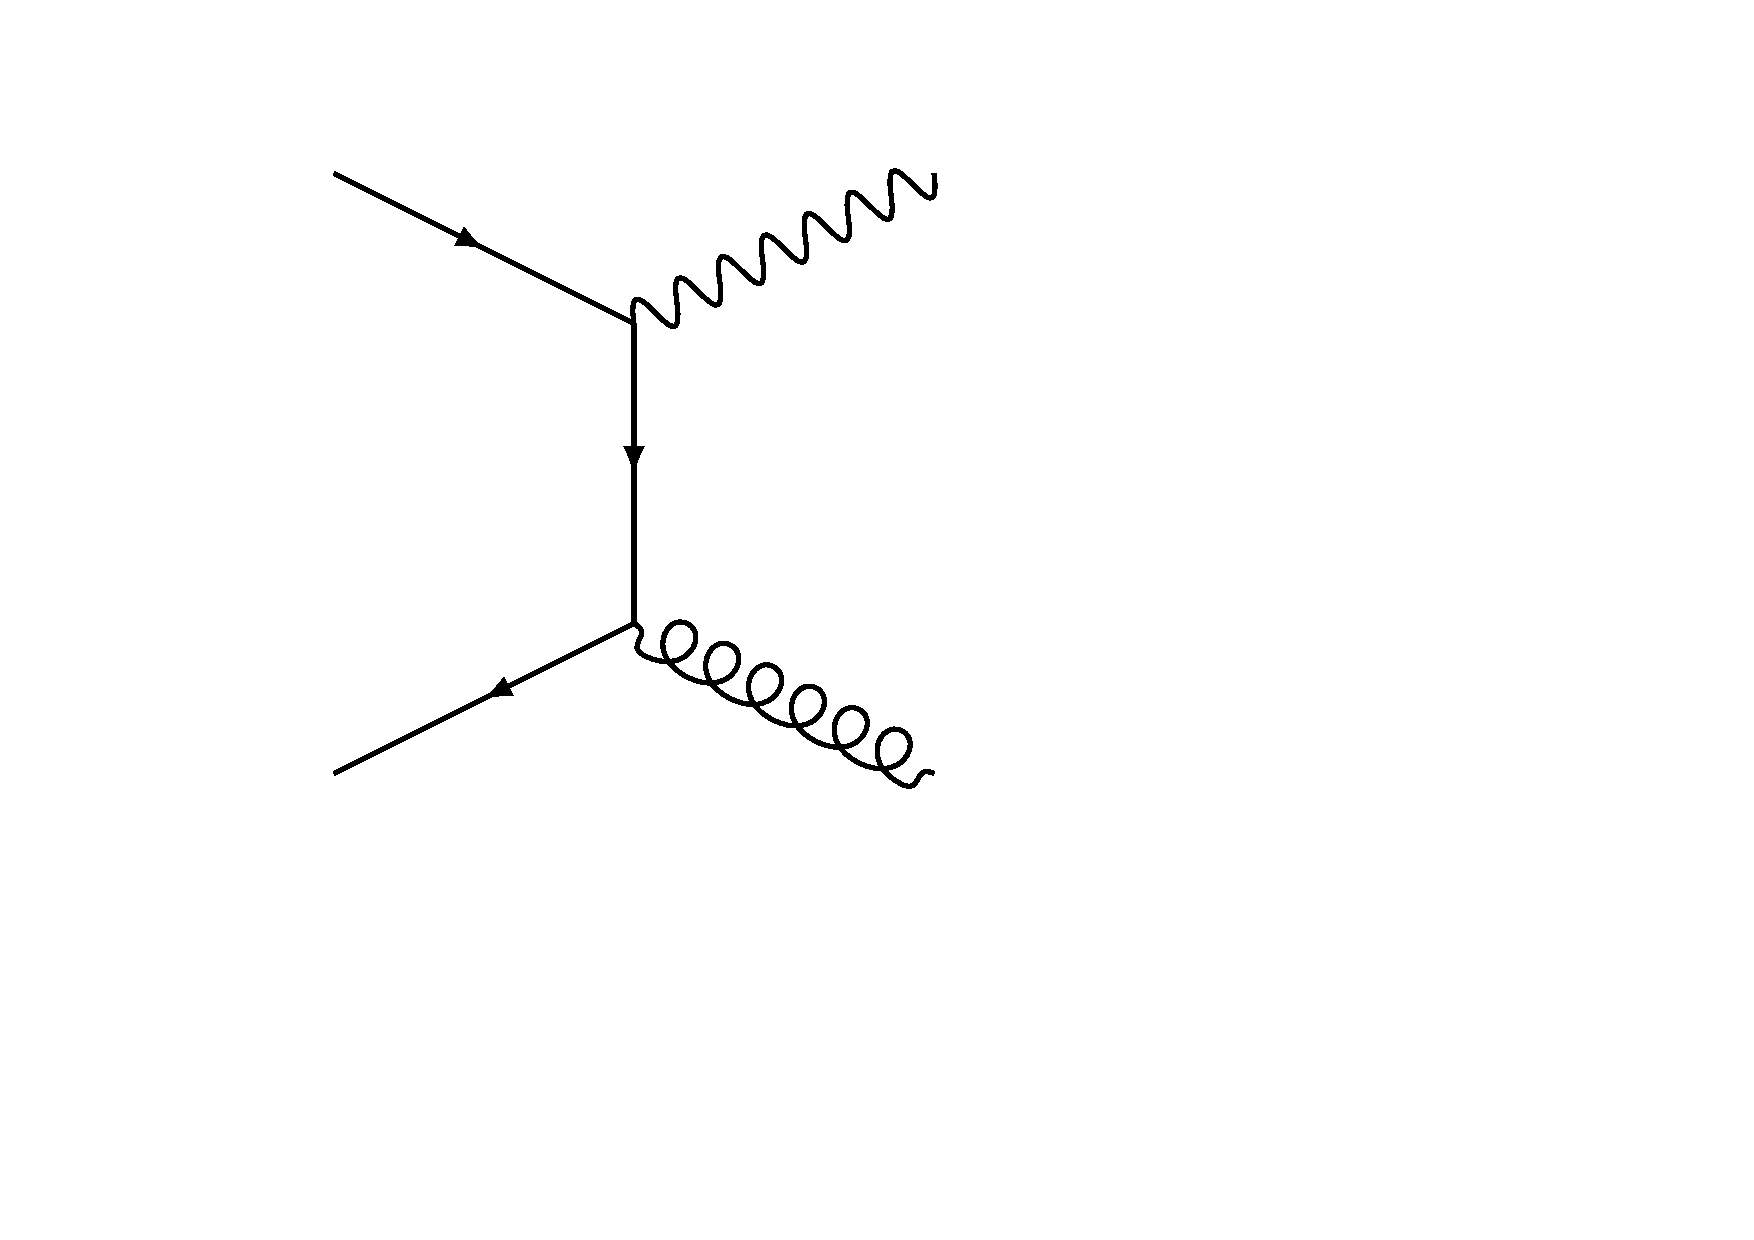
\includegraphics[width=0.25\textwidth]{figures/susy_common/feynman/W_2}\label{fig:W_prod_2}} 
\caption{\gls{lo} Feynman diagrams for the production of a W boson in associatino with one jet.}\label{fig:W_prod}
\end{figure}

\subsection{Boson Pair Production}

Beside the production of a single vector boson, also a pair production is possible.
The \gls{lo} Feynman diagrams for the production of a boson pair are shown in Fig. \ref{fig:dib_prod}.

\begin{figure}[h]
\centering 
\subfigure[]{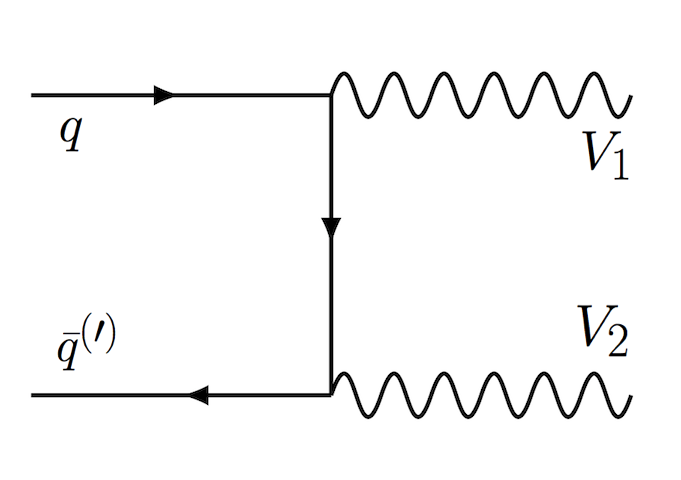
\includegraphics[width=0.3\textwidth]{figures/susy_common/feynman/dib_1}\label{fig:dib_prod_1}}
\subfigure[]{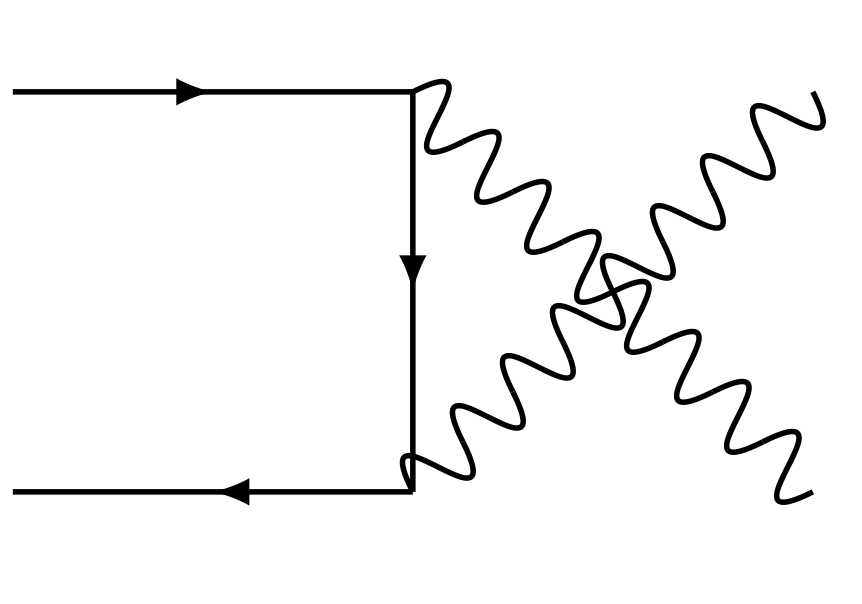
\includegraphics[width=0.3\textwidth]{figures/susy_common/feynman/dib_2}\label{fig:dib_prod_2}} 
\subfigure[]{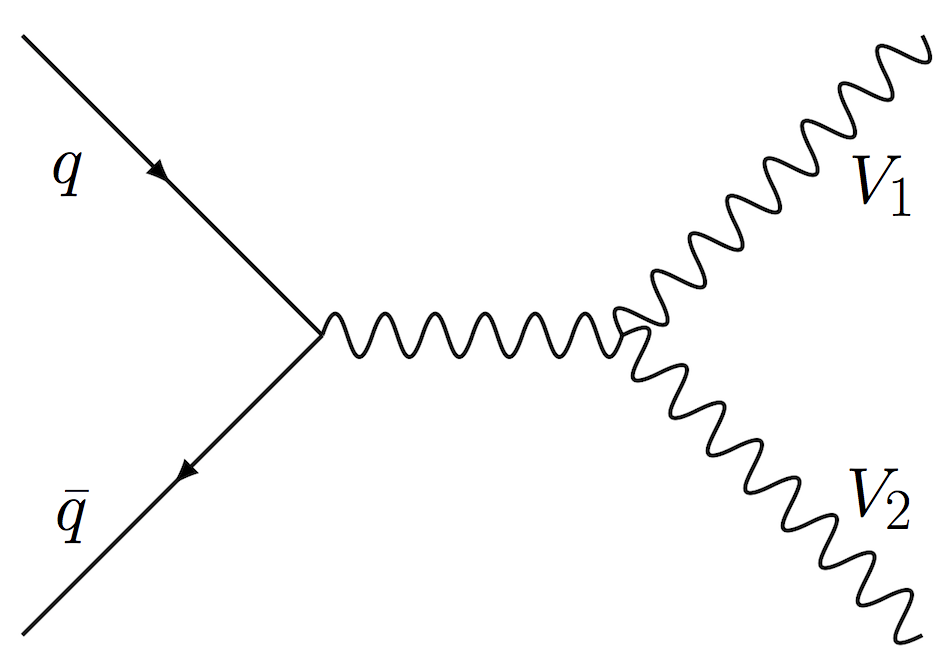
\includegraphics[width=0.3\textwidth]{figures/susy_common/feynman/dib_3}\label{fig:dib_prod_3}}
\caption{\gls{lo} Feynman diagrams for the production of a boson pair.}\label{fig:dib_prod}
\end{figure}


\subsection{\ttbar + X Production}

\begin{figure}[h]
\centering 
\subfigure[]{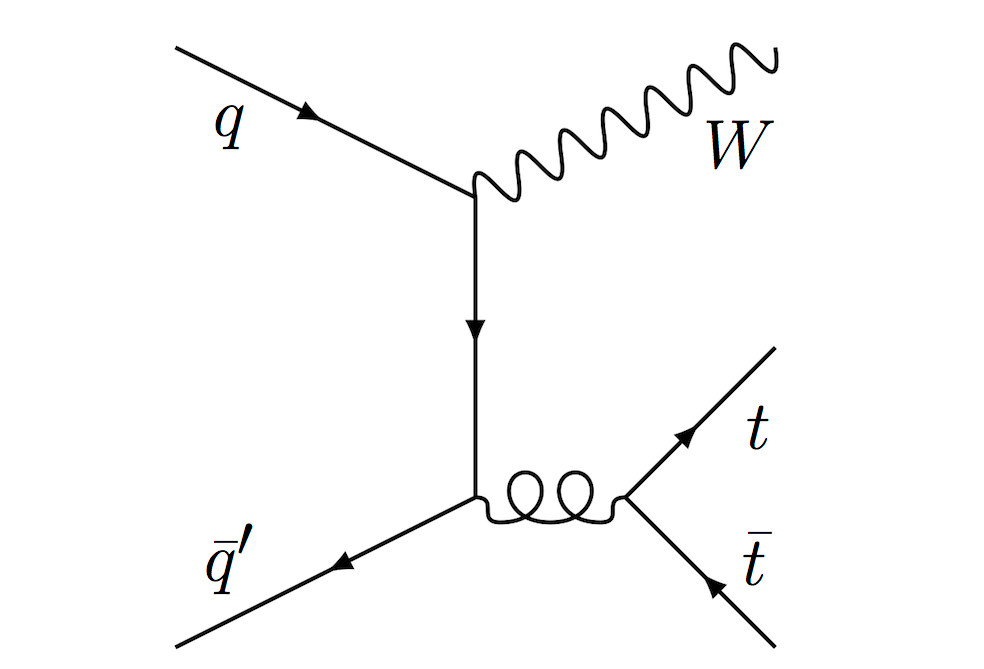
\includegraphics[width=0.3\textwidth]{figures/susy_common/feynman/ttW}\label{fig:ttW_prod}}
\subfigure[]{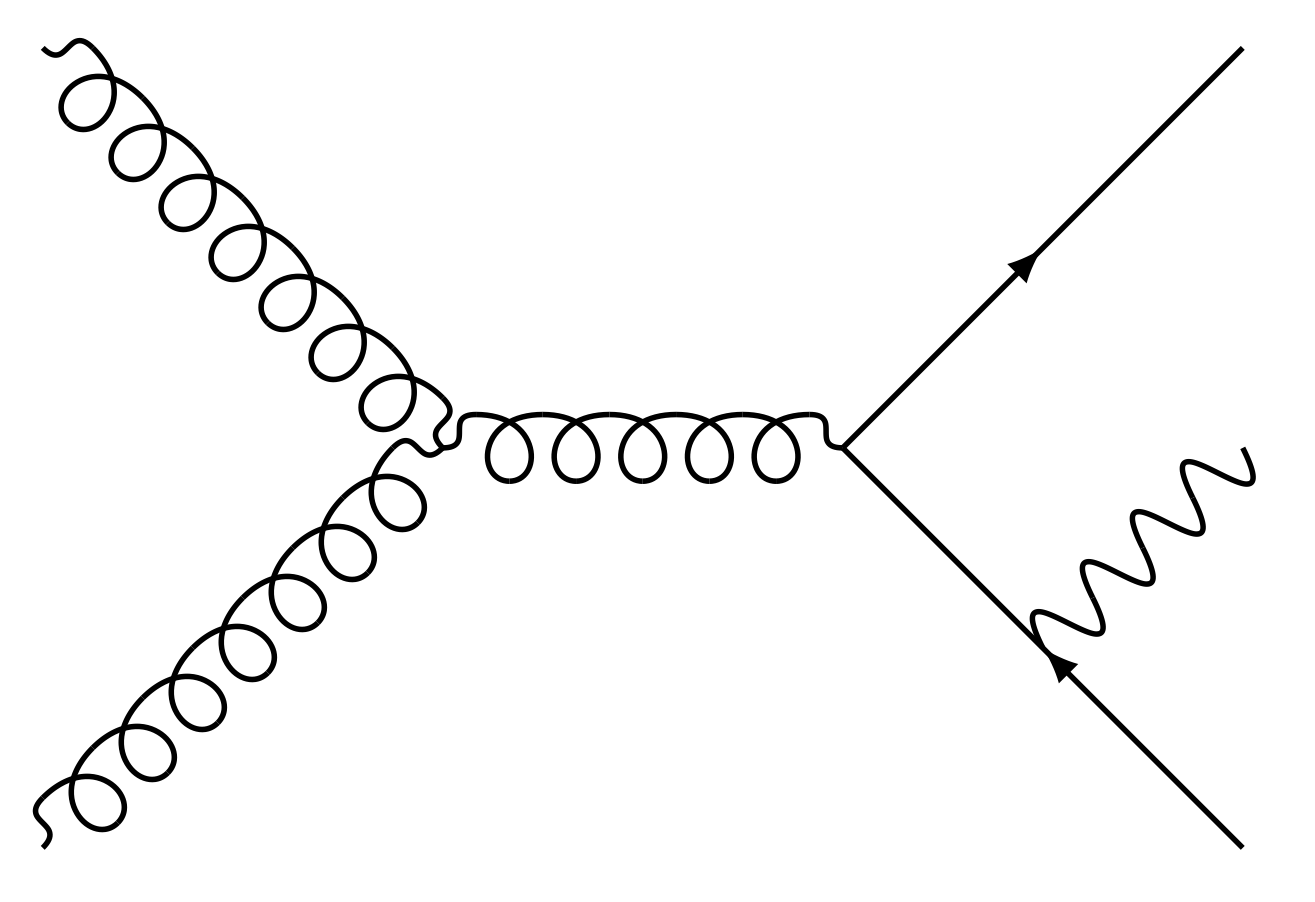
\includegraphics[width=0.3\textwidth]{figures/susy_common/feynman/ttZ}\label{fig:ttZ_prod}} \\
\subfigure[]{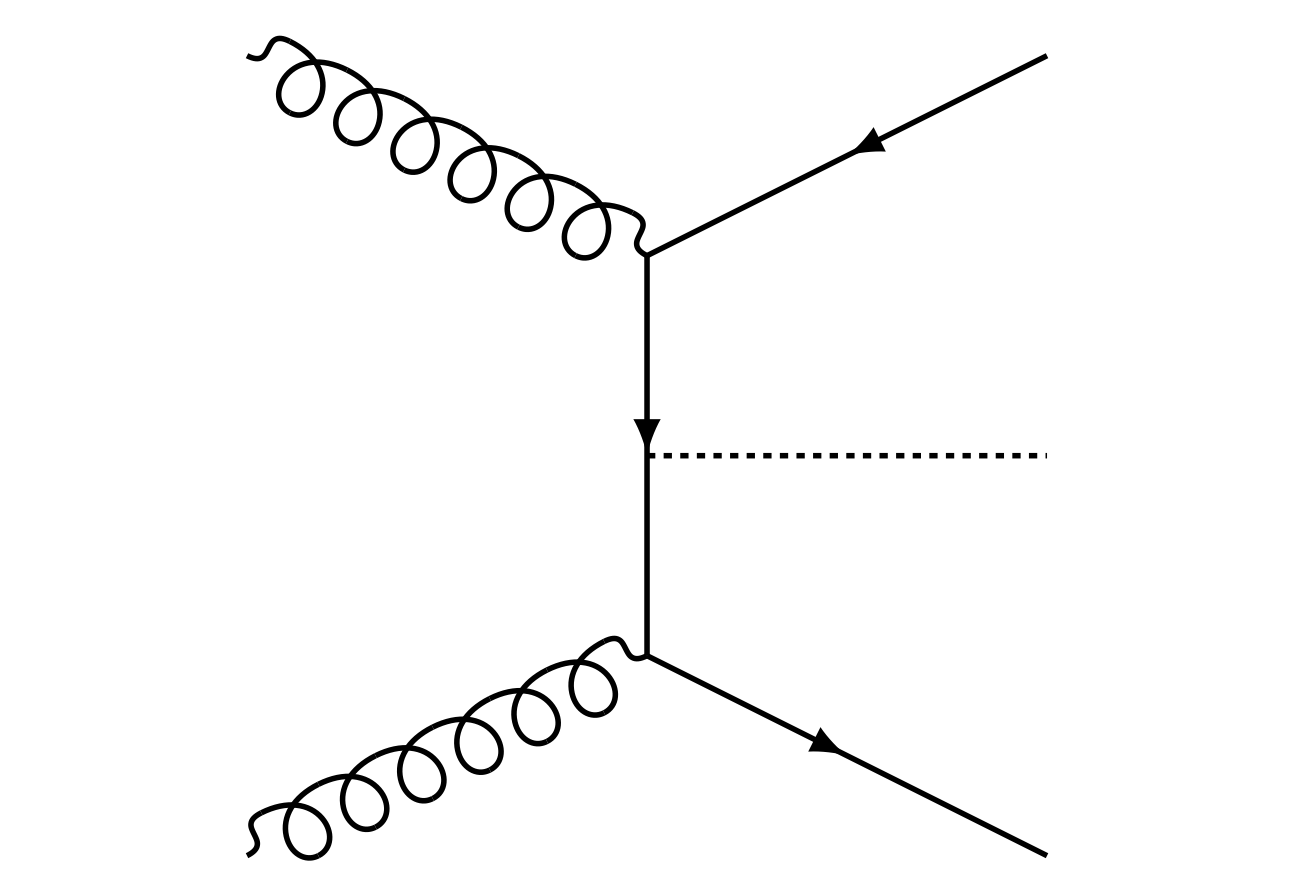
\includegraphics[width=0.3\textwidth]{figures/susy_common/feynman/tth}\label{fig:tth_prod}}
\subfigure[]{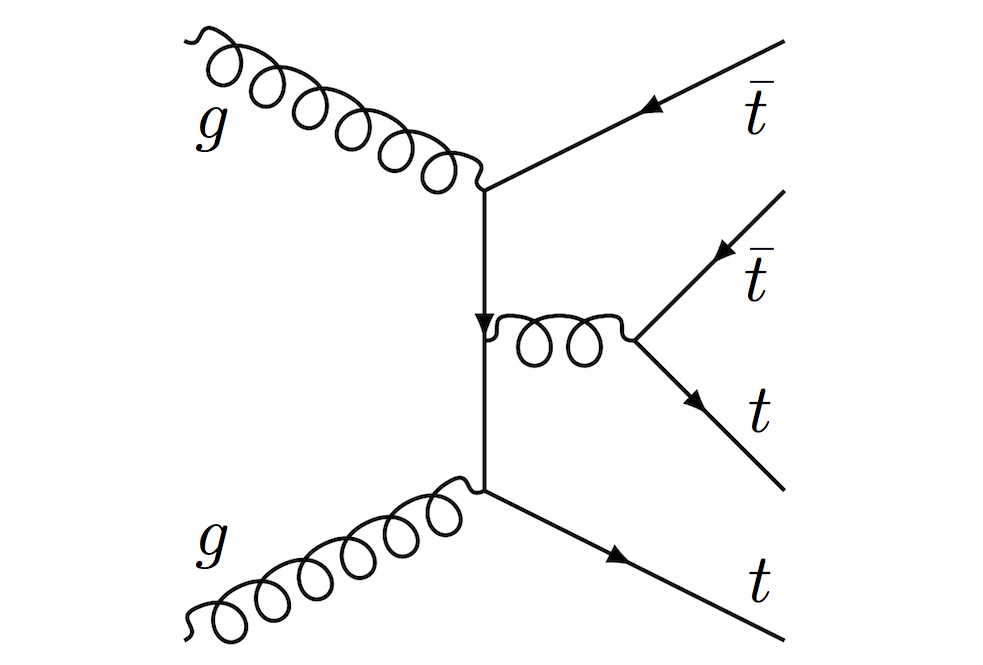
\includegraphics[width=0.3\textwidth]{figures/susy_common/feynman/fourtop}\label{fig:fourtop_prod}}
\caption{\Gls{lo} Feynman diagram for the production of \subref{fig:ttW_prod} ttW, \subref{fig:ttZ_prod} ttZ, \subref{fig:tth_prod} tth, \subref{fig:fourtop_prod} \fourtop.}\label{fig:ttX_prod}
\end{figure}

\subsection{QCD Multi-jet}

Multi-jet production is by far the process with the largest cross-section at the \gls{lhc} ($\mathcal{O}$(mb)). 
Most of the \gls{qcd} events are $2 \to 2$ processes, for which some example \gls{lo} Feynman diagrams are shown in Fig. \ref{fig:qcd_prod_1} and Fig \ref{fig:qcd_prod_2}, but higher order processes ($2 \to n$) are possible as well (an example of $2 \to 3$ process is shown in Fig. \ref{fig:qcd_prod_3}). 
Multi-jet processes do not have real \met, and therefore can be a background in analyses that require high \met only if one or more of the jets are mismeasured, leading to an energy imbalance in the transverse plane that is reconstructed as \met. 
These processes do not produce any lepton either, so also a contribution to analyses requiring leptons must origin from a jet misreconstructed as a lepton. 
Since the probability for a multi-jet event to both have a fake high \met and a fake lepton is very small, multi-jet processes are considered as background only in the analysis regions with a veto on the presence of leptons. 


\begin{figure}[h]
\centering 
\subfigure[]{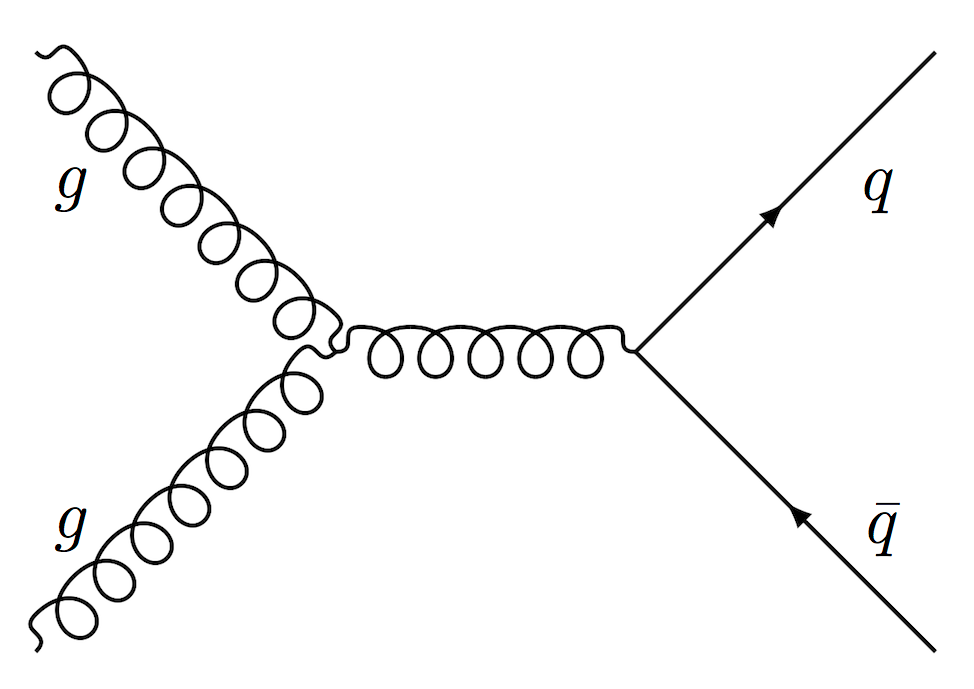
\includegraphics[width=0.3\textwidth]{figures/susy_common/feynman/qcd_1}\label{fig:qcd_prod_1}}
\subfigure[]{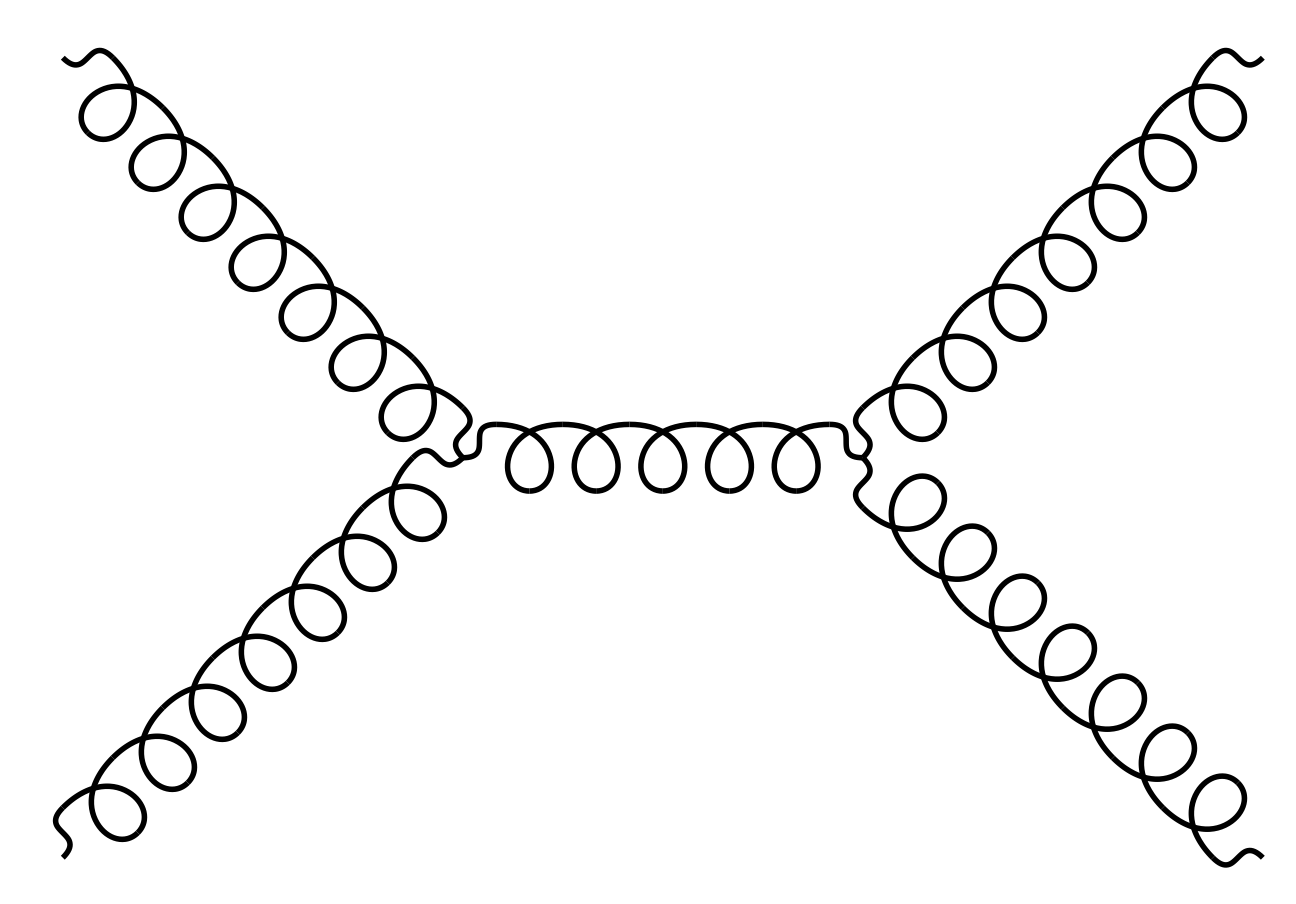
\includegraphics[width=0.3\textwidth]{figures/susy_common/feynman/qcd_2}\label{fig:qcd_prod_2}} 
\subfigure[]{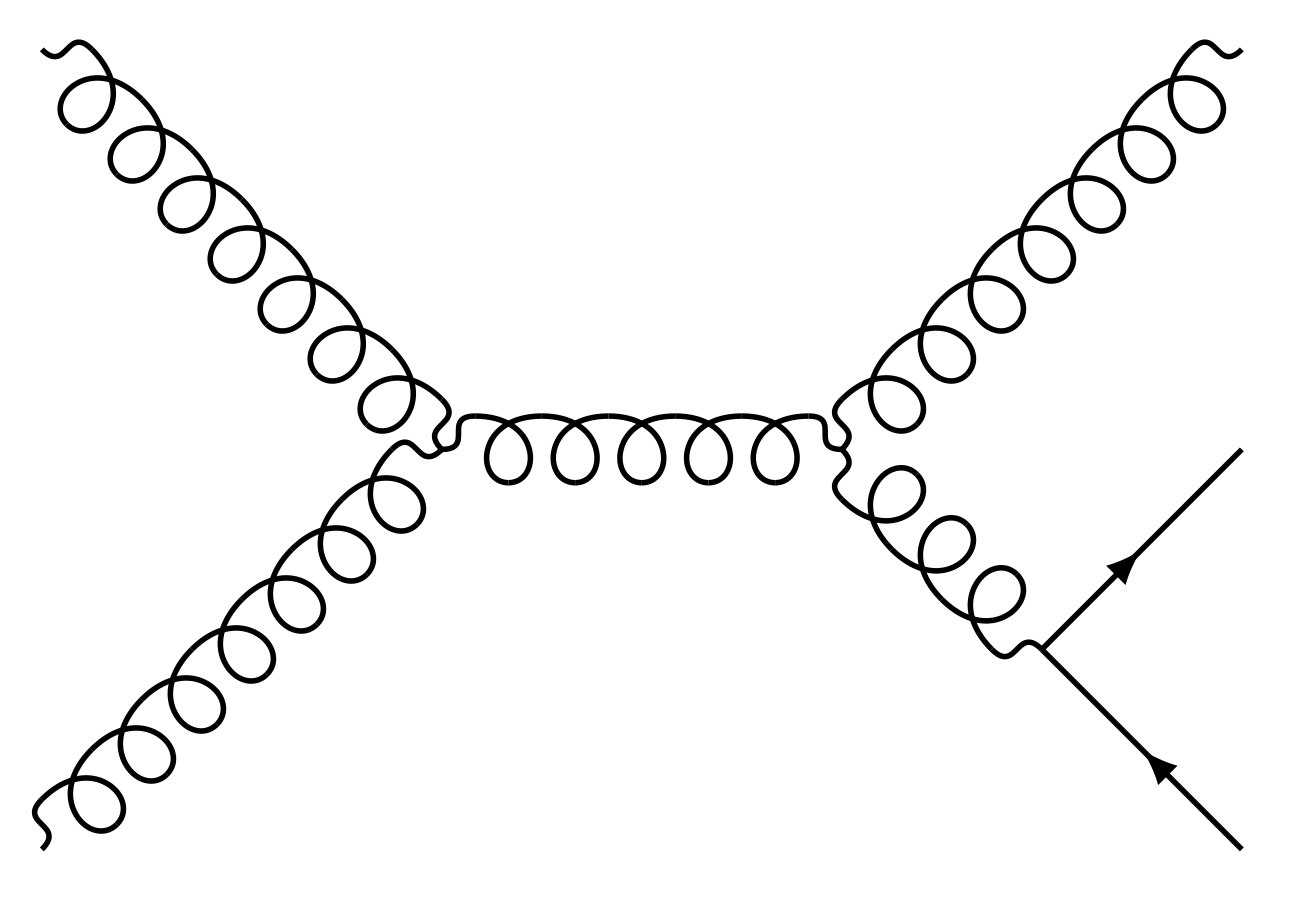
\includegraphics[width=0.3\textwidth]{figures/susy_common/feynman/qcd_3}\label{fig:qcd_prod_3}}
\caption{Example Feynman diagram for single multi-jet production. \subref{fig:qcd_prod_1}-\subref{fig:qcd_prod_2} \gls{lo} $2 \to 2$ process. 
\subref{fig:qcd_prod_3} \gls{lo} $2 \to 3$ process.}\label{fig:qcd_prod}
\end{figure}

\subsubsection{Jet Smearing}
\label{sec:jet_smearing}

The usage of \gls{mc} simulation to model the multi-jet background presents two main drawbacks.
First of all, the production cross-section for multi-jet production is very difficult to access. 
It is feasible to model the $2 \to 2$ di-jet production, 
but every additional parton in a $2 \to n$ process brings into the computation a further $\alpha_{\rm{s}}$ factor, 
and the energy scale of the interaction is low enough to be at the limit of the validity of the perturbative expansion, limiting the validity of the \gls{lo} order computation. The inclusion of corrections of higher order can improve the description, but the number of extra diagrams that should be included makes this option unrealistic (just the \gls{lo} computation for the $2 \to 2$ process only comprises 10 different diagrams).

A second problem is of practical nature: the high cross-section for multi-jet production implies a huge number of \gls{mc} events that need to be simulated in order not to have a huge statistical uncertainty. 


\section{Object Definition}
\label{sec:common_obj_def}

\section{Systematic Uncertainties}
\label{sec:common_syst}

\subsection{Experimental Systematic Uncertainties}

\subsection{Modeling Uncertainties} 

